\documentclass[a4paper]{article}
\usepackage[margin=3.5cm]{geometry}
\usepackage{amsmath}
\usepackage{amssymb}
\usepackage[svgnames]{xcolor}
\usepackage{amsthm}
% \makeatletter
% \def\th@plain{%
%   \thm@notefont{}% same as heading font
%   \itshape % body font
% }
% \def\th@definition{%
%   \thm@notefont{}% same as heading font
%   \normalfont % body font
% }
% \makeatother
\usepackage{dsfont}
\usepackage{graphicx}
\usepackage{caption}
\usepackage{hyperref}
\usepackage{cleveref}
\usepackage{datetime}
\usepackage{outlines}
\usepackage{float}
\usepackage{booktabs}
\usepackage{enumitem}
\usepackage{tabto}
\usepackage{mathtools}
\usepackage{nicematrix}
\usepackage{nccmath}
\usepackage{lipsum}
\usepackage[activate={true,nocompatibility},final,tracking=true,kerning=true,spacing=true,factor=500,stretch=15,shrink=15]{microtype}

\usepackage{apptools}
\AtAppendix{\counterwithin{lemma}{section}}

\addtolength{\skip\footins}{2mm}

\definecolor{fgcolor}{rgb}{0.345, 0.345, 0.345}
\newcommand{\hlnum}[1]{\textcolor[rgb]{0.686,0.059,0.569}{#1}}%
\newcommand{\hlstr}[1]{\textcolor[rgb]{0.192,0.494,0.8}{#1}}%
\newcommand{\hlcom}[1]{\textcolor[rgb]{0.678,0.584,0.686}{\textit{#1}}}%
\newcommand{\hlopt}[1]{\textcolor[rgb]{0,0,0}{#1}}%
\newcommand{\hlstd}[1]{\textcolor[rgb]{0.345,0.345,0.345}{#1}}%
\newcommand{\hlkwa}[1]{\textcolor[rgb]{0.161,0.373,0.58}{\textbf{#1}}}%
\newcommand{\hlkwb}[1]{\textcolor[rgb]{0.69,0.353,0.396}{#1}}%
\newcommand{\hlkwc}[1]{\textcolor[rgb]{0.333,0.667,0.333}{#1}}%
\newcommand{\hlkwd}[1]{\textcolor[rgb]{0.737,0.353,0.396}{\textbf{#1}}}%
\let\hlipl\hlkwb

\usepackage{framed}
\makeatletter
\newenvironment{kframe}{%
 \def\at@end@of@kframe{}%
 \ifinner\ifhmode%
  \def\at@end@of@kframe{\end{minipage}}%
  \begin{minipage}{\columnwidth}%
 \fi\fi%
 \def\FrameCommand##1{\hskip\@totalleftmargin \hskip-\fboxsep
 \colorbox{shadecolor}{##1}\hskip-\fboxsep
     % There is no \\@totalrightmargin, so:
     \hskip-\linewidth \hskip-\@totalleftmargin \hskip\columnwidth}%
 \MakeFramed {\advance\hsize-\width
   \@totalleftmargin\z@ \linewidth\hsize
   \@setminipage}}%
 {\par\unskip\endMakeFramed%
 \at@end@of@kframe}
\makeatother

\definecolor{shadecolor}{rgb}{.97, .97, .97}
\definecolor{messagecolor}{rgb}{0, 0, 0}
\definecolor{warningcolor}{rgb}{1, 0, 1}
\definecolor{errorcolor}{rgb}{1, 0, 0}
\newenvironment{knitrout}{}{} % an empty environment to be redefined in TeX


% code highlighting
\usepackage{minted}
\usepackage{xpatch}
\newminted[cminted]{python}{fontsize=\small}
\xpretocmd{\cminted}{\RecustomVerbatimEnvironment{Verbatim}{BVerbatim}{}}{}{}

% link coloring
\hypersetup{
   colorlinks,
   linkcolor={red!90!black},
   citecolor={green!40!black},
   urlcolor={blue!60!black}
}

% concatenation symbol (c.f. ++ in Haskell)
\newcommand\mdoubleplus{\mathbin{+\mkern-10mu+}}

% end of proof symbol
\newcommand{\newmarkedtheorem}[1]{%
  \newenvironment{#1}
    {\pushQED{\qed}\csname inner@#1\endcsname}
    {\popQED\csname endinner@#1\endcsname}%
  \newtheorem{inner@#1}%
}
% \renewenvironment{proof}{{\noindent\bfseries Proof.}}{*something*}
%\let\oldproofname=\proofname
%\renewcommand{\proofname}{\rm\bf{\oldproofname}}


\theoremstyle{definition}
%\newtheorem{eg}{Example}[section]
\newmarkedtheorem{eg}{Example}[section]
\newtheorem{remark}{Remark}
\theoremstyle{plain}
\newtheorem{define}{Definition\hspace{0.25em}\ignorespaces}
\newtheorem{property}{Property\hspace{0.25em}\ignorespaces}
\newtheorem{observation}{Observation}
\newtheorem{proposition}{Proposition}
\newtheorem{lemma}{Lemma\hspace{0.25em}\ignorespaces}
\newtheorem{corollary}{Corollary}
\newtheorem{theorem}{Theorem\hspace{0.25em}\ignorespaces}
\newtheorem{assump}{Assumption\hspace{0.25em}\ignorespaces}

\DeclareMathOperator{\interior}{int}
\newcommand*\diff{\mathop{}\!\mathrm{d}}

% cref settings
\crefname{equation}{equation}{equations}
\newcommand{\crefrangeconjunction}{--}

\newdateformat{monthyeardate}{\monthname[\THEMONTH] \THEYEAR}

\author{Jeroen van Riel}
\date{\monthyeardate\today}

\title{Trajectory optimization for vehicles in a lane model with minimum
  following distance and boundary conditions}

\begin{document}

\maketitle

\begin{abstract}
  This section considers a model of a single-lane road on which overtaking is
  not allowed.
  %
  Vehicles are modeled as double integrators with bounds on speed and
  acceleration. Consecutive vehicles must keep some fixed \textit{following
    distance} to avoid collisions.
  %
  It is assumed that vehicles enter and exit the lane at
  predetermined \textit{schedule times}. Whenever a vehicle enters or exits, it
  must drive at full speed.
  %
  For an optimization objective that, roughly speaking, minimizes the distance
  to the end of the lane at all times, we present an algorithm to compute an
  optimal set of trajectories.
  %
  Assuming some minimum lane length, we characterize feasibility of this
  trajectory optimization problem in terms of a system of linear inequalities
  involving the schedule times.
  %
\end{abstract}

% \tableofcontents

\newcommand\halfopen[2]{\ensuremath{[#1,#2)}}
\newcommand\openhalf[2]{\ensuremath{(#1,#2]}}

\renewcommand{\labelitemii}{\textbullet}
\renewcommand{\labelitemiii}{\textbullet}

\section{Lane model}

Vehicles are modeled as double integrators with bounded speed and acceleration,
which means that we only consider their longitudinal position on the road. Let
$\mathcal{D}[a,b]$ denote the set of valid \emph{trajectories}, which we define to be
all continuously differentiable functions $x : [a,b] \rightarrow \mathbb{R}$ satisfying
the constraints
\begin{align}
  0 \leq \dot{x}(t) \leq 1 \quad \text{ and } \quad
  {-\omega} \leq \ddot{x}(t) \leq \bar{\omega} , \quad \text{ for all } t \in [a,b] ,
\end{align}
for some fixed acceleration bounds $\omega, \bar{\omega} > 0$. Note that we use $\dot{x}$
and $\ddot{x}$ to denote the first and second derivative with respect to time
$t$. When we have a general positive speed upper bound, we can always apply an
appropriate scaling of the time axis and the acceleration bounds to obtain the
form.
%
Consider positions $A, B \in \mathbb{R}$, such that $B \geq A$, which denote the
start\footnote{We could have assumed $A=0$, but we will later piece together
  multiple lanes to model intersections.} and end position of the lane.
%
Let $\bar{D}[a, b] \subset \mathcal{D}[a, b]$ denote the set of trajectories $x$ that
satisfy the boundary conditions
\begin{align}
  x(a) = A \; \text{ and } \; x(b) = B .
\end{align}
Even further, let $D[a,b] \subset \bar{D}[a, b]$ induce the boundary conditions
\begin{align}
  \dot{x}(a) = \dot{x}(b) = 1 .
\end{align}
In words, these boundary conditions require that a vehicle arrives to and
departs from the lane at predetermined times $a$ and $b$ and do so at full
speed.

Let $L > 0$ denote the required \textit{following distance} between consecutive
vehicles.
%
Suppose we have $N$ vehicles that are scheduled to traverse the lane. For each
vehicle $i$, let $a_{i}$ and $b_{i}$ denote the \textit{schedule time} for entry
and exit, respectively. A feasible solution consists of a sequence of
trajectories $x_{1}, \dots, x_{N}$ such that
\begin{subequations}\label{eq:feasibility}
\begin{align}
x_{i} \in D[a_{i}, b_{i}] \quad \quad & \text{ for each } i, \\
x_{i} \leq x_{i-1} - L \quad \quad &\text{ for each } i \geq 2,
\end{align}
\end{subequations}
%
where we use the shorthand notation $\gamma_{1} \leq \gamma_{2}$ to mean
$\gamma_{1}(t) \leq \gamma_{2}(t)$ for all
$t \in [a_{1}, b_{1}] \cap [a_{2}, b_{2}]$, given some
$\gamma_{1} \in \mathcal{D}[a_{1}, b_{1}]$ and
$\gamma_{2} \in \mathcal{D}[a_{2}, b_{2}]$.
% We use $\gamma \leq \min \{ \gamma_{1}, \dots, \gamma_{n} \}$ as a shorthand for $\gamma \leq \gamma_{1}, \dots, \gamma \leq \gamma_{n}$.

As optimization objective, we will consider
\begin{align}\label{eq:objective}
  \max \; \sum_{i=1}^{N} \int_{a_{i}}^{b_{i}} x_{i}(t) \diff t ,
\end{align}
which, roughly speaking, seeks to keep all vehicles as close to the end of the
lane at all times.
%
In particular, we will show that optimal trajectories can be understood as the
concatenation of at most four different types of trajectory parts. Based on this
observation, we present an algorithm to compute optimal trajectories.
%
Assuming $(\omega, \bar{\omega},A,B,L)$ to be fixed, with lane length $B-A$
sufficiently large, we will show that feasibility of the trajectory optimization
problem is completely characterized by a system of linear inequalities in
$a_{i}$ and $b_{i}$.

Note that objective~\eqref{eq:objective} does not capture energy efficiency in
any way. Although this is not desirable in practice, it is precisely this
assumption that enables the analysis in this section. Deriving a similar
characterization of feasibility and optimal trajectories under an objective that
does model energy concumption is an interesting topic for further research.

\section{Single vehicle problem}

We will first consider a somewhat generalized version of the
constraints~\eqref{eq:feasibility} for a single vehicle $i$. Therefore, we
lighten the notation slightly by dropping the vehicle index $i$ and instead of
$x_{i-1} - L$, we assume we are given some arbitrary \emph{lead vehicle
  boundary} $\bar{x} \in \bar{D}[\bar{a}, \bar{b}]$, then we consider the
optimization problem
\begin{align}
  \max_{x \in D[a, b]} \int_{a}^{b} x(t) \diff t \quad \text{ such that } \quad x \leq \bar{x} .
\end{align}
to which we will refer as the \emph{single vehicle problem}.

\subsection{Necessary conditions}

For every trajectory $x \in D[a,b]$, we derive two upper
bounding trajectories $x^{1}$ and $\hat{x}$ and one lower bounding trajectory
$\check{x}$, see Figure~\ref{fig:necessary-conditions}.
%
Using these bounding trajectories, we will then formulate four necessary
conditions for feasibility of the single vehicle problem.

Let the \emph{full speed boundary} $x^{1}$ be defined as
\begin{align}
  x^{1}(t) = A + t - a,
\end{align}
for all $t \in [a, b]$, then we clearly have $x \leq x^{1}$.
%
Next, since deceleration is at most $\omega$, we have
$\dot{x}(t) \geq \dot{x}(a) - \omega(t - a) = 1 - \omega(t - a)$, which we
combine with the speed constraint $\dot{x} \geq 0$ to derive
$\dot{x}(t) \geq \max\{0, 1 - \omega (t - a) \}$. Hence, we obtain the lower
bound
\begin{align}\label{eq:check-x}
  x(t) = x(a) + \int_{a}^{t} \dot{x}(\tau) \diff \tau \geq A + \int_{a}^{t} \max\{0, 1 - \omega (\tau - a) \} \diff \tau =: \check{x}(t) .
\end{align}
%
Analogously, we derive an upper bound from the fact that acceleration is at most $\bar{\omega}$. Observe that we have
$\dot{x}(t) + \bar{\omega} (b - t) \geq \dot{x}(b) = 1$, which we combine
with the speed constraint $\dot{x}(t) \geq 0$ to derive
$\dot{x}(t) \geq \max \{ 0, 1 - \bar{\omega}(b - t) \}$. Hence, we obtain the
upper bound
\begin{align}\label{eq:hat-x}
  x(t) = x(b) - \int_{t}^{b} \dot{x}(\tau) \diff \tau
  \leq B - \int_{t}^{b} \max\{ 0, 1 -\bar{\omega} (b - \tau) \} \diff \tau =: \hat{x}(t) .
\end{align}
%
We refer to $\check{x}$ and $\hat{x}$ as the \emph{entry boundary} and
\emph{exit boundary}, respectively.


\begin{figure}
  \centering
  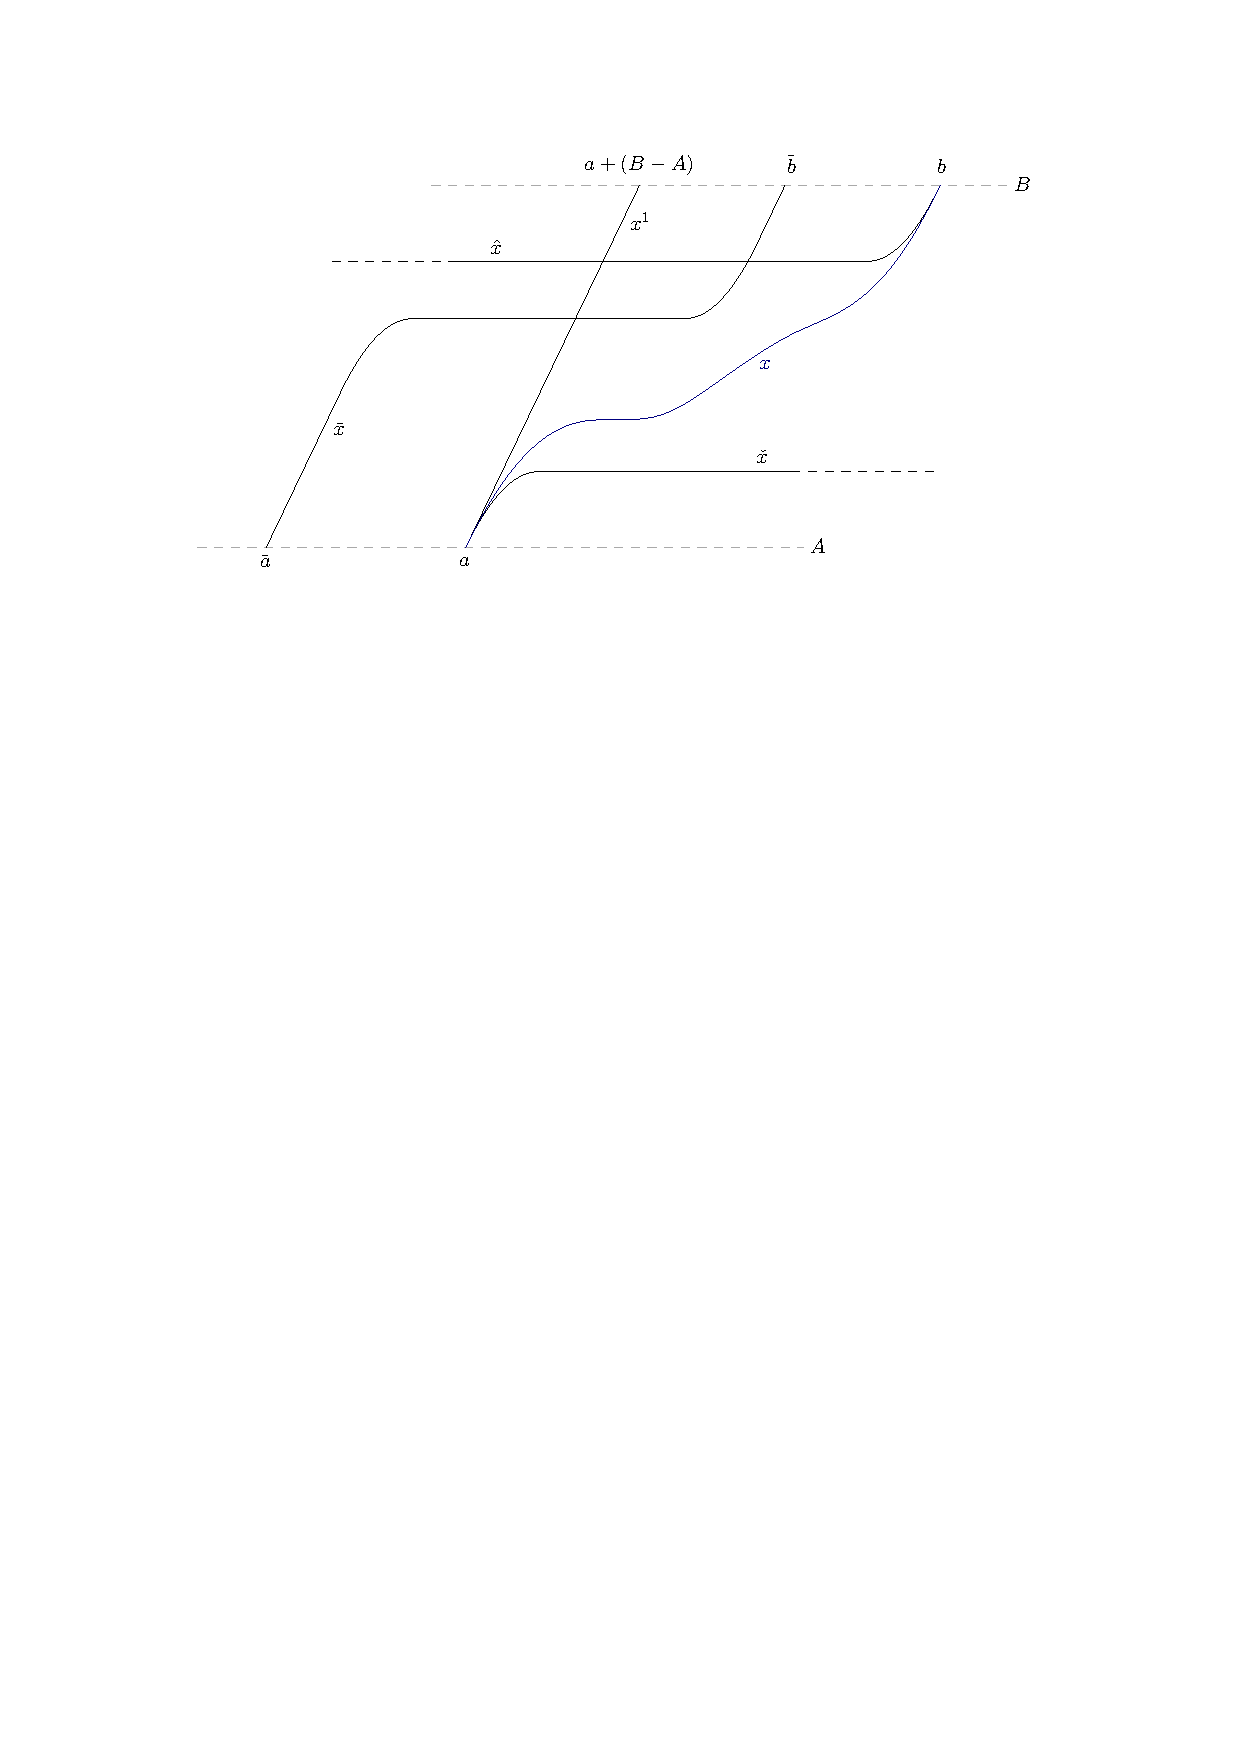
\includegraphics[scale=1]{figures/motion/rough/necessary-conditions}
  \caption{Illustration of the four bounding trajectories
    $\bar{x}, x^{1}, \hat{x}, \check{x}$ that bound feasible trajectories from
    above and below. We also drew an example of a feasible trajectory $x$ in
    blue. The horizontal axis represents time and the vertical axis corresponds
    to the position on the lane, so the vertical dashed grey lines correspond to
    the start and end of the lane.}%
  \label{fig:necessary-conditions}
\end{figure}

\pagebreak

\begin{lemma}\label{lemma:necessary-conditions}
  Let $\bar{x} \in \bar{D}[\bar{a}, \bar{b}]$ and assume there exists a
  trajectory $x \in D[a, b]$ such that $x \leq \bar{x}$, then the following
  conditions must hold \TabPositions{3cm}
  \begin{enumerate}[label=(\roman*)\quad,leftmargin=5em]
    \item $b-a \geq B-A$, \tab (full speed constraint)
    \item $\bar{b} \leq b$, \tab (downstream order constraint)
    \item $\bar{a} \leq a$, \tab (upstream order constraint)
    \item $\bar{x} \geq \check{x}$. \tab (entry space constraint)
  \end{enumerate}
\end{lemma}
\begin{proof}
  Each of the conditions corresponds somehow to one of the four bounding
  trajectories defined above.
  %
  Observe that $x^{1}(t) = B$ for $t = a + (B-A)$, which can be interpreted as
  the earliest time of departure from the lane. This shows that
  $b \geq a + (B-A)$, which is equivalent with (i).
  %
  % When (i) is violated, $x$ must cross $x^{1}$ somewhere, which means that the
  % maximum speed constraint must be violated.
  When either (ii) or (iii) is violated, the constraint $x \leq \bar{x}$
  conflicts with one of the boundary conditions $x(a) = A$ or $x(b) = B$. To see
  that (iv) must hold, suppose that $\bar{x}(\tau) < \check{x}(\tau)$ for some
  time $\tau$. Since $\bar{a} \leq a$, this means that $\bar{a}$ must intersect
  $\check{a}$ from above. Therefore, any trajectory that satisfies
  $x \leq \bar{x}$ must also intersect $\check{a}$ from above, which contradicts
  the assumption that $x$ was a feasible solution.
\end{proof}

We show that the boundaries $\hat{x}$ and $\check{x}$ together could yield yet
another necessary condition. It is straightforward to verify
from~\cref{eq:hat-x,eq:check-x} that $\hat{x}(t) \geq B - 1/(2\bar{\omega})$ and
$\check{x}(t) \leq A + 1/(2\omega)$. Therefore, whenever
$B - A < 1/(2\bar{\omega}) + 1/(2\omega)$, these boundaries intersect for
certain values of $a$ and $b$. Because the exact condition is somewhat
cumbersome to characterize, we avoid this case by simply assuming that the lane
length is sufficiently large.

\begin{assump}\label{eq:AB-assumption}
  The length of the lane satisfies $B - A \geq 1/(2\omega) + 1/(2\bar{\omega})$.
\end{assump}

\pagebreak

\subsection{Constructing the optimal trajectory}

Assuming the four conditions of Lemma~\ref{lemma:necessary-conditions} hold, we will construct an optimal
solution $x^{*}$ for the single vehicle problem, thereby showing that these
conditions are thus also sufficient for feasibility.
%
First, we construct $x^{*}$ by combining the upper boundaries $\bar{x}$,
$\hat{x}$ and $x^{1}$ in a certain way to obtain a smooth trajectory satisfying
$x^{*} \in D[a,b]$.
%
We show that $x^{*}$ is still an upper boundary for any other feasible solution,
which shows that it is optimal.

\begin{figure}
  \centering
  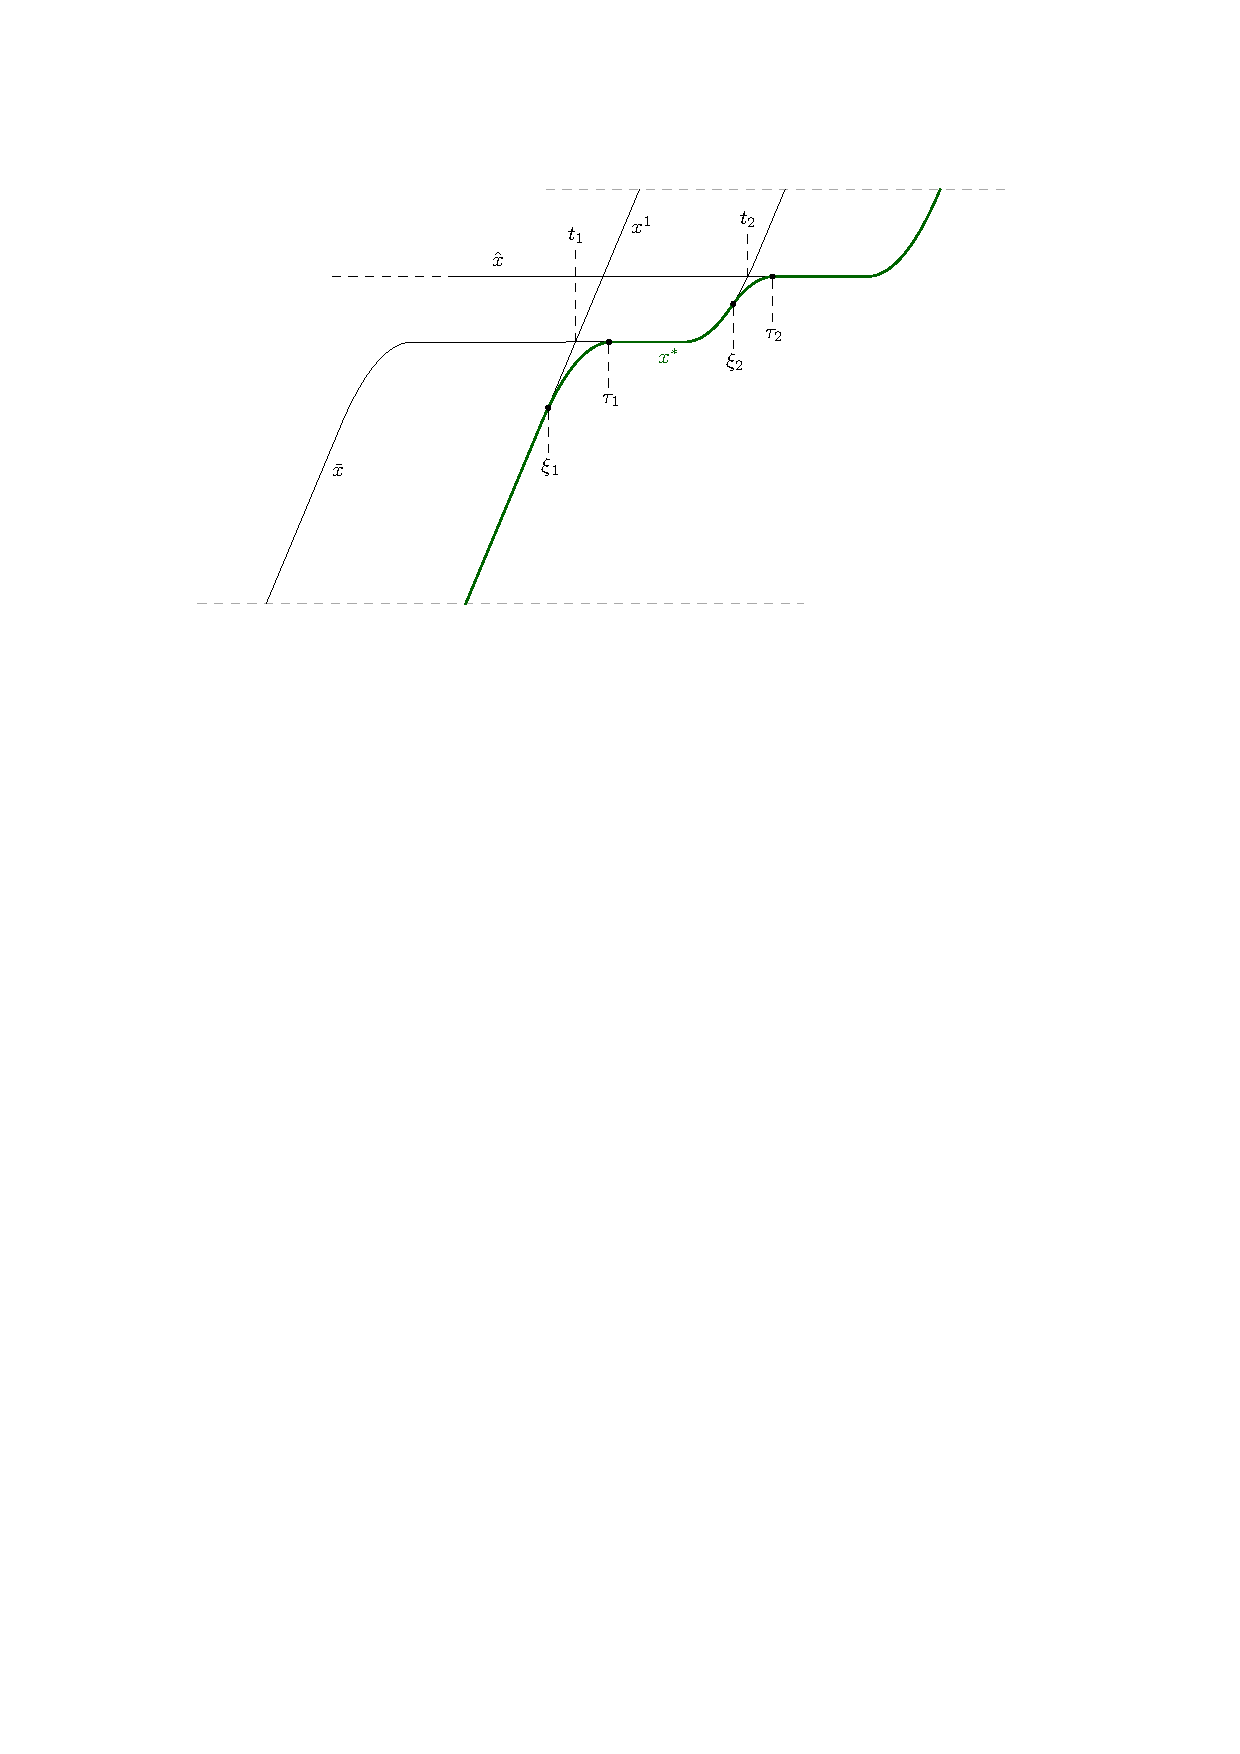
\includegraphics[scale=1]{figures/motion/rough/proof}
  \caption{The minimum boundary $\gamma$, induced by three upper boundaries
    $\bar{x}$, $\hat{x}$ and $x^{1}$, is smoothened around time $t_{1}$ and
    $t_{2}$, where the derivative is discontinuous, to obtain the smooth optimal
    trajectory $x^{*}$, drawn in green.}%
  \label{fig:optimal-construction}
\end{figure}

The starting point of the construction is the \emph{minimum boundary}
$\gamma : [a,b] \rightarrow \mathbb{R}$ induced by the upper boundaries, defined as
\begin{align}\label{eq:min-boundary}
  \gamma(t) := \min \{ \bar{x}(t), \hat{x}(t), x^{1}(t) \} .
\end{align}
%
Obviously, $\gamma$ is still a valid upper boundary for any feasible solution,
%
but in general, $\gamma$ may have a discontinuous derivative at some\footnote{In fact, it can be shown that, under the necessary conditions, there are at most two of such discontinuities.} isolated
points in time.

\begin{define}\label{def:piecewise-trajectory}
  Let $\mathcal{P}[a,b]$ be the set of functions $\mu : [a, b] \rightarrow \mathbb{R}$ for
  which there is a finite subdivision $a = t_{0} < \cdots < t_{n+1} = b$ such that
  the truncation $\mu|_{[t_{i}, t_{i+1}]} \in \mathcal{D}[t_{i}, t_{i+1}]$ is
  a smooth trajectory, for each $i \in \{0, \dots, n\}$, and for which the one-sided limits of $\dot{\mu}$ satisfy
  \begin{align}
    \dot{\mu}(t_{i}^{-}) := \lim_{t \uparrow t_{i}} \dot{\mu}(t) > \lim_{t \downarrow t_{i}} \dot{\mu}(t) =: \dot{\mu}(t_{i}^{+}) ,
  \end{align}
  for each $i \in \{1, \dots, n\}$. We refer to such $\mu$ as a \emph{piecewise
    trajectory (with downward bends)}.
\end{define}

It is not difficult to see from Figure~\ref{fig:necessary-conditions} that,
under the necessary conditions, $\gamma$ satisfies the above definition, so
$\gamma \in \mathcal{P}[a,b]$. In other words, $\gamma$ consists of a number of
pieces that are smooth and satisfy the vehicle dynamics, with possibly some
sharp bend downwards where these pieces come together.
%
Next, we present a simple procedure to smoothen out this kind of discontinuity
by decelerating from the original trajectory somewhat before some $t_{i}$, as
illustrated in Figure~\ref{fig:optimal-construction}. We show that this procedure can be repeated at every
point of discontinuity.

\subsubsection{Deceleration boundary}
In order to formalize the smoothing procedure, we will first define some
parameterized family of functions to model the deceleration part.
%
Recall the derivation of $\check{x}$ in equation~\eqref{eq:check-x} and the discussion
preceding it, which we will now generalize a bit.
%
Let $x \in \mathcal{D}[a, b]$ be some smooth trajectory, then observe that $\dot{x}(t) \geq \dot{x}(\xi) - \omega(t - \xi)$ for all $t \in [a, b]$.
Combining this with the constraint $\dot{x}(t) \in [0, 1]$, this yields
\begin{align}
  \dot{x}(t) \geq \max\{ 0, \, \min\{1, \, \dot{x}(\xi) - \omega (t - \xi) \}\} =: \{\dot{x}(\xi) - \omega(t-\xi)\}_{[0,1]} ,
\end{align}
where use $\{ \cdot \}_{[0,1]}$ as a shorthand for this clipping operation.
%
Hence, for any $t \in [a,b]$, we obtain the following lower bound
\begin{align}\label{eq:stopping-trajectory}
  x(t) = x(\xi) + \int_{\xi}^{t} \dot{x}(\tau) \diff \tau \geq x(\xi) + \int_{\xi}^{t} \{\dot{x}(\xi) - \omega(\tau - \xi)\}_{[0,1]} \diff \tau =: x[\xi] (t) ,
\end{align}
where we will refer to the right-hand side as the \emph{deceleration boundary} of $x$
at $\xi$.

Note that $x[\xi]$ depends on $x$ only through the two real numbers $x(\xi)$ and
$\dot{x}(\xi)$. It will be convenient later to rewrite the right-hand side
of~\eqref{eq:stopping-trajectory} as
\begin{align}
  x^{-}[p, v, \xi](t) = p + \int_{\xi}^{t} \{ v - \omega(\tau - \xi) \}_{[0,1]} \diff \tau ,
\end{align}
such that $x[\xi](t) = x^{-}[x(\xi), \dot{x}(\xi), \xi](t)$.
%
We can expand the integral in this expression further by carefully handling
the clipping operation. Observe that the expression within the clipping
operation reaches the bounds $1$ and $0$ for $\delta_{1} := \xi - (1-v)/\omega$ and
$\delta_{0} := \xi + v/\omega$, respectively. Using this notation, a simple calculation
shows that
\begin{align}\label{eq:x-}
  x^{-}[p,v,\xi](t) = p +
  \begin{cases}
    {(1 - v)}^{2} / (2\omega) + (t - \xi) & \text{ for } t \leq \delta_{1} , \\
    v(t - \xi) - \omega{(t-\xi)}^{2} /2 & \text{ for } t \in [\delta_{1} , \delta_{0}] , \\
    v^{2}/(2\omega) & \text{ for } t \geq \delta_{0} .
  \end{cases}
\end{align}
Assuming $0 \leq v \leq 1$, it can be verified that for every $t \in \mathbb{R}$, we
have $\ddot{x}^{-}[p,v,\xi](t) \in \{-\omega, 0\}$ and
$\dot{x}^{-}[p,v,\xi](t) \in [0,1]$ due to the clipping operation, so that
$x^{-}[p,v,\xi] \in \mathcal{D}(-\infty,\infty)$.

\begin{figure}
  \centering
  \includegraphics[scale=1]{figures/motion/rough/stopping-trajectory}
  \caption{Illustration of a deceleration boundary $\mu[\xi]$ of some piecewise
    trajectory $\mu \in \mathcal{P}[a,b]$ at time $\xi$. We truncated $\mu[\xi]$
    for a more compact figure. This particular trajectory $\mu$ has a
    discontinuous derivative at times $t_{1}$ and $t_{2}$. The careful reader
    may notice that this $\mu$ cannot occur as the minimum boundary defined
    in~\eqref{eq:min-boundary}. This only means that the class of piecewise
    trajectories $\mathcal{P}[a,b]$ is just slightly more general than necessary
    for our current purposes.}%
  \label{fig:stopping-trajectory}
\end{figure}

Let $\mu \in \mathcal{P}[a, b]$ be some piecewise trajectory and let
$a = t_{0} < \cdots < t_{n+1} = b$ denote the corresponding subdivision as in
Definition~\ref{def:piecewise-trajectory}, then we generalize the definition of
a deceleration boundary to $\mu$.
%
Whenever $\xi \in [a,b] \setminus \{ t_{1}, \dots, t_{n}\}$, we just define
$\mu[\xi] := x^{-}[\mu(\xi), \dot{\mu}(\xi), \xi]$.
%
However, when $\xi \in \{ t_{1}, \dots, t_{n}\}$, the derivative
$\dot{\mu}(\xi)$ is not defined, so we to use the left-sided limit instead, by
defining $\mu[\xi] := x^{-}[\mu(\xi), \dot{\mu}(\xi^{-}), \xi]$.
%
Finally, please note that we cannot just replace $x$ with $\mu$ in
inequality~\eqref{eq:stopping-trajectory} to obtain a similar bound for the
whole interval $[a,b]$.
%
Instead, consider some interval
$I \in \{ [a, t_{1}], \openhalf{t_{1}}{t_{2}}, \dots, \openhalf{t_{n}}{b} \}$,
then what remains true is that $\xi \in I$ implies $\mu(t) \geq \mu[\xi](t)$ for
every $t \in I$.


\subsubsection{Smoothing procedure}
Let $\mu \in \mathcal{P}[a,b]$ be some piecewise trajectory and let
$a = t_{0} < \cdots < t_{n+1} = b$ again denote the subdivision as in Definition~\ref{def:piecewise-trajectory}.
%
We first show how to smoothen the discontinuity at $t_{1}$ and then we argue how
to repeat this process for the remaining times $t_{i}$.

\begin{assump}
  Throughout the following discussion, we assume $\mu \geq \mu[a]$ and $\mu \geq \mu[b]$.
\end{assump}

We want to pick some $\xi \in \halfopen{a}{t_{1}}$, such that $\mu[\xi] \leq \mu$
and such that $\mu[\xi]$ touches $\mu$ at some time $\tau \in [t_{1}, b]$
tangentially. Therefore, we measure the relative position of $\mu[\xi]$ with
respect to $\mu$ on this interval, by considering
\begin{align}
  d(\xi) := \min_{t \in [t_{1}, b]} \mu(t) - \mu[\xi](t) .
\end{align}
Since $\mu(t)$ and $\mu[\xi](t)$ are both continuous in $t$, this minimum actually exists
due to the extreme value theorem (Weierstrass).
%
Furthermore, since the minimum is taken of a continuous function over a closed
interval, $d$ is a continuous function as well (see Lemma~\ref{lemma:inf-continuous}).

Observe that $d(a) \geq 0$, because $\mu \geq \mu[a]$ by assumption.
%
By definition of $t_{1}$, we have $\dot{\mu}(t_{1}^{-}) > \dot{\mu}(t_{1}^{+})$,
from which it follows that $\mu < \mu[t_{1}]$ on $(t_{1}, t_{1} + \epsilon)$ for some small
$\epsilon > 0$, which shows that $d(t_{1}) < 0$.
%
Therefore, the intermediate value theorem ensures that there is some
$\xi_{1} \in \halfopen{a}{t_{1}}$ such that $d(\xi_{1}) = 0$.

Next, we are going to show that $\mu[\xi_{1}]$ is unique. More precisely, for
any $\xi \in \halfopen{a}{t_{1}}$ such that $d(\xi) = 0$, we have
$\mu[\xi] = \mu[\xi_{1}]$.
%
The first step is to establish that the level set
\begin{align}
  X := \{ \xi \in \halfopen{a}{t_{1}} : d(\xi) = 0 \}
\end{align}
is a closed interval. To this end, we show that $d$ is non-increasing on
$\halfopen{a}{t_{1}}$, which together with continuity implies the desired result
(see Lemma~\ref{lemma:levelset}).
%
To show that $d$ is non-increasing, it suffices to show that $\mu[\xi](t)$ is
non-decreasing as a function of $\xi$, for every $t \in [t_{1}, b]$.
%
Therefore, we compute the partial derivative of $\mu[\xi]$ with respect to
$\xi$.
%
Recall the definition of $\mu[\xi]$ based on the definition of $x^{-}$ in
equation~\eqref{eq:x-}.
%
Using the same notation, we write
$\delta_{1} = \xi - (1 - \dot{\mu}(\xi))/\omega$ and
$\delta_{0} = \xi + \dot{\mu}(\xi)/\omega$ and compute
%
\begin{align}
  \frac{\partial}{\partial \xi} \mu[\xi](t) =
  \dot{\mu}(\xi) +
  \begin{cases}
    \ddot{\mu}(\xi)(\dot{\mu}(\xi)-1)/\omega - 1 &\text{ for } t \leq \delta_{1} , \\
    \ddot{\mu}(\xi)(t-\xi) - \dot{\mu}(\xi) + \omega(t-\xi) &\text{ for } t \in [\delta_{1},\delta_{0}] , \\
    \ddot{\mu}(\xi)\dot{\mu}(\xi)/ \omega &\text{ for } t \geq \delta_{0} .
  \end{cases}
\end{align}
%
It is easily verified that these three cases match at $\delta_{1}$ and
$\delta_{0}$. Now consider any $\xi \in \halfopen{a}{t_{1}}$ and
$t \in [t_{1}, b]$, then we have $\delta_{1} \leq \xi \leq t$, so we only have
to verify the second and third case.
%
In the second case, we have
$\dot{\mu}(\xi) + \ddot{\mu}(\xi)(t-\xi) - \dot{\mu}(\xi) + \omega(t-\xi) = (\ddot{\mu}(\xi) + \omega)(t-\xi) \geq 0$.
%
The third case gives
$\dot{\mu}(\xi) + \ddot{\mu}(\xi)\dot{\mu}(\xi)/\omega \geq \dot{\mu}(\xi) + (-\omega)\dot{\mu}(\xi)/\omega = 0$.

\begin{outline}
  \1 Show that $\mu[\xi]$ is the same, regardless of $\xi \in X$.

  \1 Let $t^{*} \in [t_{1}, b]$ be a minimizer of the minimum $d(\xi_{1}) = 0$,
  such that $\mu(t^{*}) = \mu[\xi_{1}](t^{*})$.
  %
  If $\tau_{1} \in (t_{1}, b)$, then obviously
  $\dot{\mu}(\tau_{1}) = \dot{\mu}[\xi_{1}](\tau_{1})$ is a necessary condition
  of a local minimum. Note that $\tau_{1}=t_{1}$ cannot happen.

  \1 When $\tau_{1} = b$, the derivatives must match as a consequence of
  assumption $\mu \geq \mu[b]$.

  \1 Conclude that we have found a $\xi, \tau$ such that the boundary
  $\mu[\xi]_{[\xi,\tau]}$ can be added to $\mu$ to obtain
  $\mu' \in \mathcal{P}[a,b]$ with one less discontinuity. For $\mu'$, we can
  repeat the exact same process as above. Eventually, we end up with a
  trajectory $\mu^{*} \in \mathcal{D}[a,b]$.

  \1 Argue that the smoothing procedure leaves $\dot{\mu}^{*}(a) = \dot{\mu}(a)$
  and $\dot{\mu}^{*}(b) = \dot{\mu}(b)$ untouched.
\end{outline}


\subsubsection{Optimality after smoothing}


{\color{Navy} Observe that the necessary conditions require $\gamma(a) = A$,
  $\gamma(b) = B$ and $\dot{\gamma}(a) = \dot{\gamma}(b) = 1$, so whenever we
  have $\gamma \in \mathcal{D}[a, b]$, we automatically have $\gamma \in D[a,b]$
  so that $\gamma$ is already an optimal solution. }

\begin{lemma}\label{lemma:upperbound}
  Let $\mu \in \mathcal{P}[a,b]$ be a piecewise trajectory and let
  $\mu^{*} \in \mathcal{D}[a,b]$ denote the result after smoothing. All
  trajectories $x \in \mathcal{D}[a, b]$ that are such that
  $x \leq \mu$, must satisfy $x \leq \mu^{*}$.
\end{lemma}
\begin{proof}
  Consider the interval $(\xi, \tau)$ of a joining deceleration part. Suppose
  there exists some $t_{d} \in (\xi, \tau)$ such that
  $x(t_{d}) > \mu(t_{d})$. Because $x(\xi) \leq \mu(\xi)$, this means
  that $x$ must intersect $\mu$ at least once in $\halfopen{\xi}{t_{d}}$,
  so let
  $t_{c} := \sup \, \{ t \in \halfopen{\xi}{t_{d}} : x(t) = \mu(t) \}$ be
  the latest time of intersection such that $x \geq \mu$ on
  $[t_{c}, t_{d}]$. There must be some $t_{c} \in [t_{c}, t_{d}]$ such that
  $\dot{x}(t_{v}) > \dot{\mu}(t_{v})$, otherwise
  \begin{align*}
    x(t_{d}) = x(t_{c}) + \int_{t_{c}}^{t_{d}} \dot{x}(t) \diff t \leq \mu(t_{c}) + \int_{t_{c}}^{t_{d}} \dot{\mu}(t) \diff t = \mu(d_{t}) ,
  \end{align*}
  which contradicts our choice of $t_{d}$. Hence, for every
  $t \in [t_{v}, \tau]$, we have
  \begin{align*}
    \dot{x}(t) \geq \dot{x}(t_{v}) - \omega (t - t_{v}) > \dot{\mu}(t_{v}) - \omega(t - t_{v}) = \dot{\mu}(t) .
  \end{align*}
  It follows that $x(\tau) > \mu(\tau)$, which contradicts the assumption.
\end{proof}

\newpage
\section{Computing optimal trajectories}

\begin{define}
  Let $\gamma \in \mathcal{D}[a, b]$ be called \emph{alternating} if for all $t \in [a, b]$,
  we have
  \begin{align}
    \ddot{\gamma}(t) \in \{-\omega, 0, \bar{\omega}\} \quad \text{ and } \quad
  \ddot{\gamma}(t) = 0 \implies \dot{\gamma}(t) \in \{0, 1\}.
  \end{align}
\end{define}

Observe that we can distinguish four consecutive phases of an alternating
trajectory: full speed $\dot{\gamma} = 1$, full deceleration
$\ddot{\gamma} = -\omega$, full stop $\dot{\gamma} = 0$ and full acceleration
$\ddot{\gamma} = \bar{\omega}$.

\begin{lemma}
  Let $\gamma_{1} \in \mathcal{D}[a_{1}, b_{1}]$ and $\gamma_{2} \in \mathcal{D}[a_{2}, b_{2}]$ be both alternating, then when $\gamma_{1} * \gamma_{2}$ exists, it is also alternating.
\end{lemma}

Derive $x^{+}$ similarly to how we derived $x^{-}$ when we introduced the
deceleration boundary.

\begin{remark}
  From the proof above, it also becomes clear that a connecting deceleration can only happen between the following four pairs of partial trajectories:
  \begin{align*}
     x^{+} \rightarrow x^{+} , \quad \quad
     x^{+} \rightarrow x^{0} , \quad \quad
     x^{1} \rightarrow x^{+} , \quad \quad
     x^{1} \rightarrow x^{0} .
  \end{align*}
\end{remark}

\section{Feasibility as system of linear inequalities}


% \begin{figure}
%   \centering
%   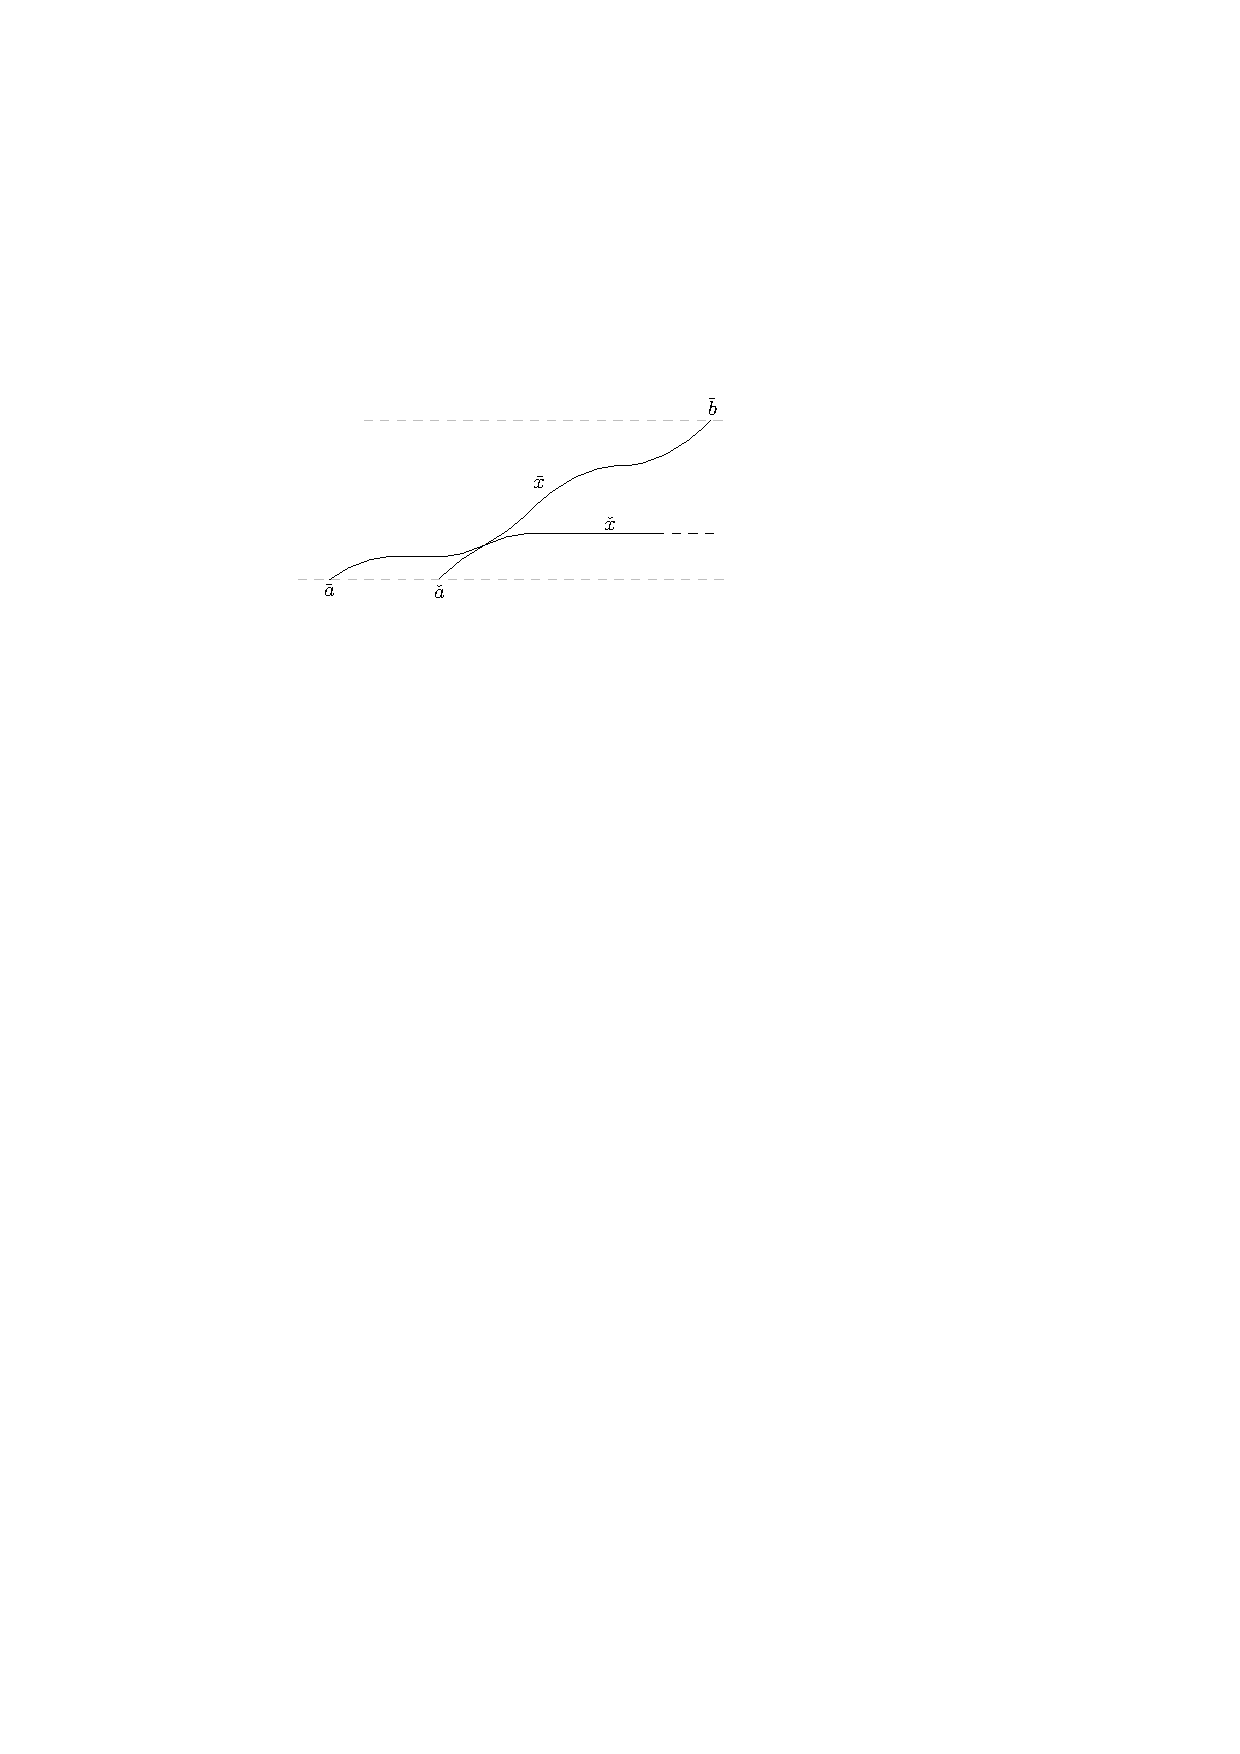
\includegraphics[scale=1]{figures/motion/rough/bufferconstraint}
%   \caption{Illustration of buffer constraint.}%
%   \label{fig:bufferconstraint}
% \end{figure}

\newpage

\begin{figure}
  \centering
  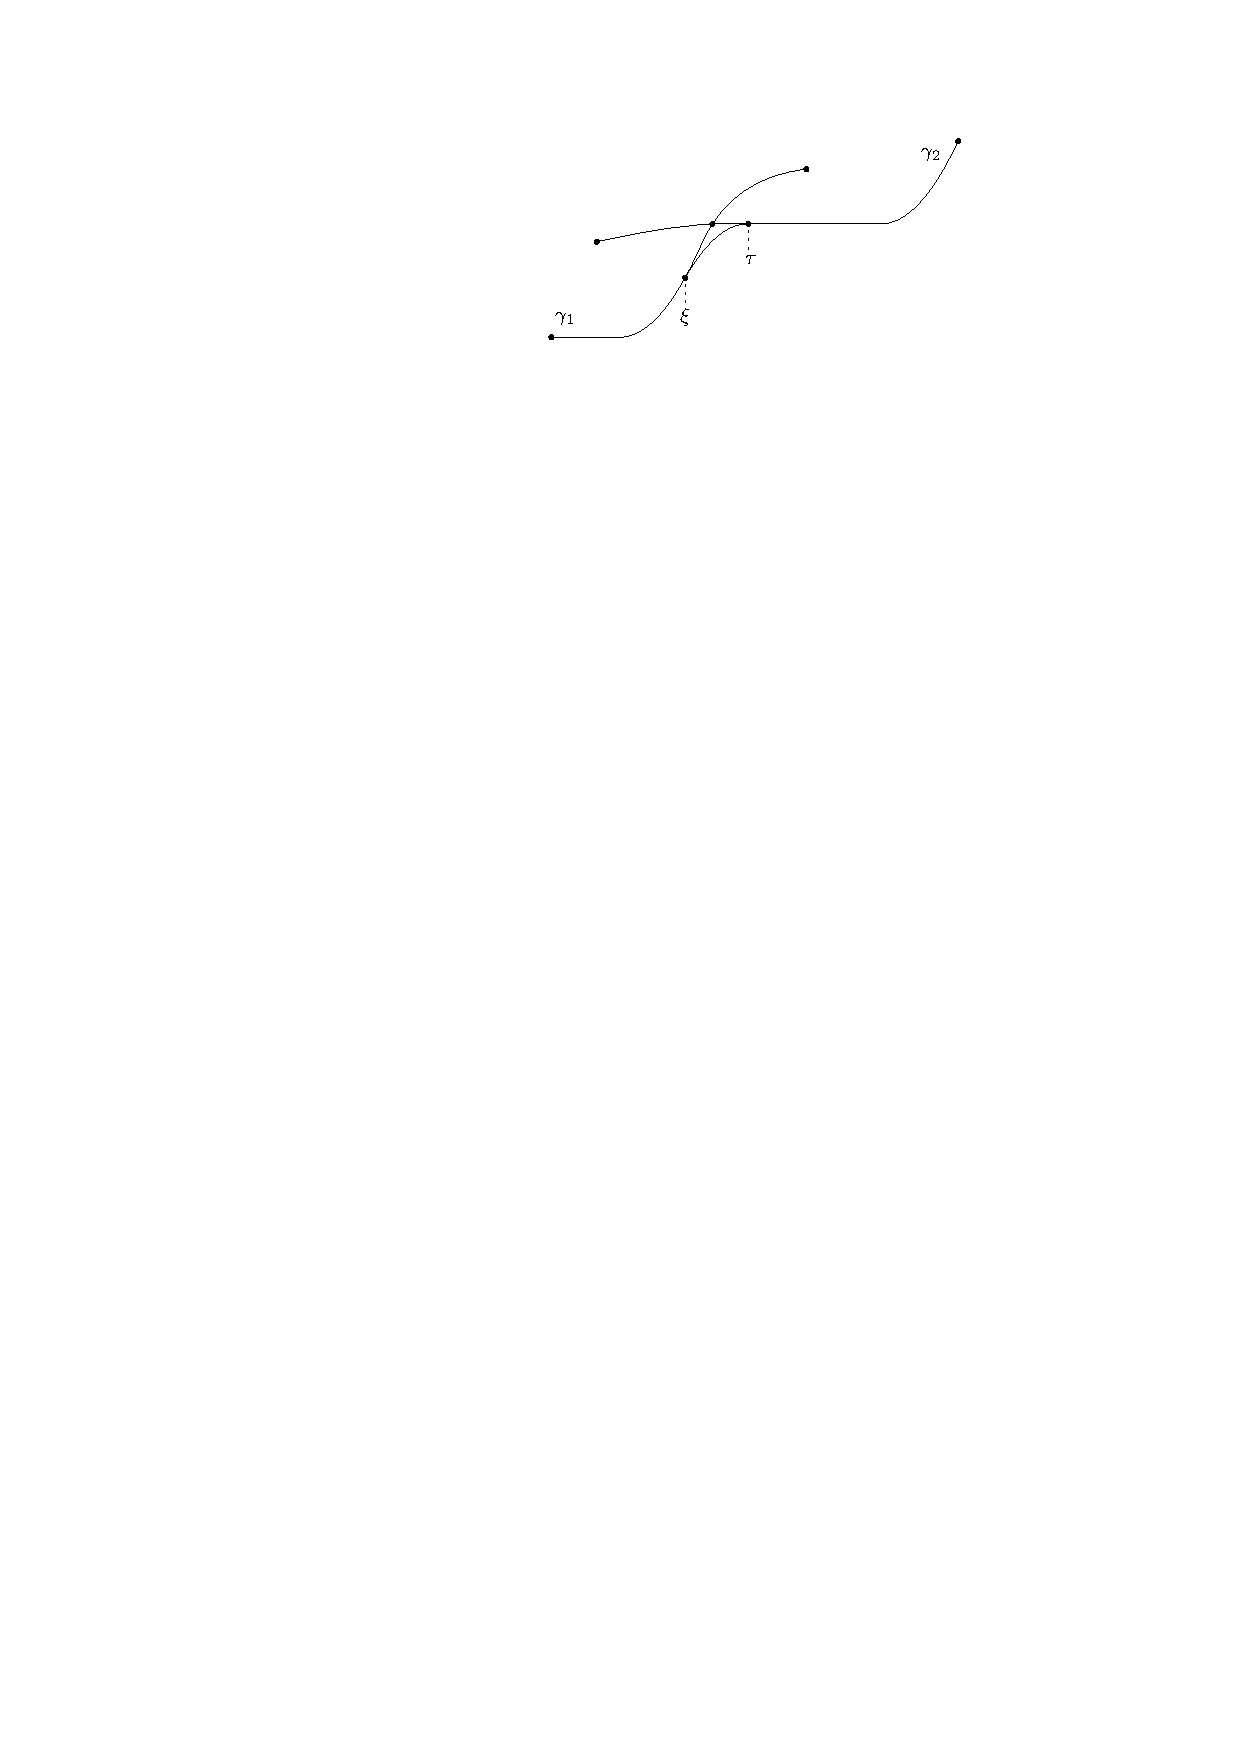
\includegraphics[scale=1]{figures/motion/rough/curvejoining}
  \caption{Two intersecting trajectories joined together by a part of a stopping
    trajectory.}%
  \label{fig:curvejoining}
\end{figure}

Consider two crossing trajectories $\gamma_{1}$ and $\gamma_{2}$ like in
Figure~\ref{fig:curvejoining}. Roughly speaking, we want to construct a new
trajectory $\mu$ by finding some times $\xi$ and $\tau$ such that
$\mu = \gamma_{1}$ until $\xi$ and $\mu = \gamma_{2}$ after $\tau$ and such that
full deceleration during the interval $[\xi, \tau]$ takes us from $\gamma_{1}$
onto $\gamma_{2}$, with matching tangents.
%
After precisely defining the kind of trajectories we allow, we show that such a
\emph{joined trajectory} is unique, when it exists. Furthermore, we provide a
condition for existence and show a certain upper bounding property, which we
will apply in the next section to characterize optimal trajectories.


Furthermore, $\gamma[\xi](t)$ is a non-decreasing function in terms of either of its
arguments, while fixing the other. To see this for $\xi$, fix any $t$ and
consider $\xi_{1} \leq \xi_{2}$, then note that $\gamma[\xi_{1}](t)$ is a lower
bound for $\gamma[\xi_{2}](t)$.
%
\begin{property}
  Both $\gamma[\xi](t)$ and $\dot{\gamma}[\xi](t)$ are continuous when considered as functions
  of $(\xi, t)$.
\end{property}
\begin{proof}
  Write $f(\xi, t) := \gamma[\xi](t)$ to emphasize that we are dealing with two variables.
  Recall that $\dot{\gamma}$ is continuous by assumption, so the equation
  $\tau = \xi + \dot{\gamma}(\xi)/\omega$ defines a separation boundary of the
  domain of $f$. Both cases of~\eqref{eq:underbound} are continuous and they
  agree at this boundary, so $f$ is continuous on all of its domain.
  %
  Since $x \mapsto \max\{0, x \}$ is continuous, it is easy to see that also
  $(\xi, t) \mapsto \dot{\gamma}[\xi](t) = \max\{0, \dot{\gamma}(\xi) - \omega (\tau - \xi) \}$
  is continuous.
\end{proof}

Because $\gamma[\xi](t)$ is continuous and non-decreasing in $\xi$, the set
\begin{align}\label{eq:X}
  X(t_{0}, x_{0}) := \{\xi : \gamma[\xi](t_{0}) = x_{0}\}
\end{align}
is a closed interval (follows from Lemma~\ref{lemma:levelset}), so we can consider the maximum
\begin{align}\label{eq:xi}
  \xi(t_{0}, x_{0}) := \max X(t_{0}, x_{0}) .
\end{align}
%
Consider the closed region $\bar{U} := \{ (t, x) : \gamma[a](t) \leq x \leq \gamma[b](t) \}$.
For each $(t_{0}, x_{0}) \in \bar{U}$, there must be some $\xi_{0}$ such that
$\gamma[\xi_{0}](t_{0}) = x_{0}$, as a consequence of the intermediate value theorem and the
above continuity property.
%
Consider $\bar{U}$ without the points on $\gamma$, which we denote by
\begin{align}\label{eq:U}
  U := \bar{U} \setminus \{ (t,x) : \gamma(t) = x\}.
\end{align}
Next, we prove that $\gamma[\xi_{0}]$ is actually unique if $(t_{0}, x_{0}) \in U$, so that we
may regard $\xi(t_{0}, x_{0})$ as the canonical representation of this unique
trajectory $\gamma[\xi(t_{0}, x_{0})]$.

\begin{property}\label{prop:xi-unique}
  For $(t_{0}, x_{0}) \in U$, if
  $\gamma[\xi_{1}](t_{0}) = \gamma[\xi_{2}](t_{0}) = x_{0}$, then
  $\gamma[\xi_{1}] = \gamma[\xi_{2}]$.
\end{property}
\begin{proof}
  Suppose $t_{0} < \xi_{i}$, then $x_{0} = \gamma[\xi_{i}](t_{0}) = \gamma(t_{0})$ contradicts the assumption $(t_{0}, x_{0}) \in U$.
  %
  Therefore, assume $\xi_{1} \leq \xi_{2} < t_{0}$, without loss of generality.
  %
  Since $\gamma[\xi_{1}] = \gamma[\xi_{2}]$ on $[a, \xi_{1}]$, note that
  we have the lower bounds
  \begin{align}\label{eq:lowerbounds}
    \gamma[\xi_{1}] \leq \gamma[\xi_{2}] \quad \text{ and } \quad \dot{\gamma}[\xi_{1}] \leq \dot{\gamma}[\xi_{2}].
  \end{align}
  %
  We must have $\dot{\gamma}[\xi_{1}](t_{0}) = \dot{\gamma}[\xi_{2}](t_{0})$,
  because otherwise $\gamma[\xi_{1}] > \gamma[\xi_{2}]$ somewhere in a
  sufficiently small neighborhood of $t_{0}$, which contradicts the first lower
  bound.

  It is clear from Definition~\ref{def:stopping-trajectory} that
  \begin{align*}
    \ddot{\gamma}[\xi_{i}](t) =
    \begin{cases}
      \ddot{\gamma}(t) & \text{ for } t < \xi_{i} , \\
      - \omega & \text{ for } t \in (\xi_{i}, \xi_{i} + \dot{\gamma}(\xi_{i})/\omega) , \\
      0 & \text{ for } t > \xi_{i} + \dot{\gamma}(\xi_{i})/ \omega ,
    \end{cases}
  \end{align*}
  for both $i \in \{ 1, 2\}$.
  %
  Note that
  $\dot{\gamma}(\xi_{1}) - \omega(\xi_{2}-\xi_{1}) \leq \dot{\gamma}(\xi_{2})$,
  which can be rewritten as
  \begin{align*}
    \xi_{2} + \dot{\gamma}(\xi_{2}) / \omega \geq \xi_{1} + \dot{\gamma}(\xi_{1}) / \omega .
  \end{align*}
  This shows that $\ddot{\gamma}[\xi_{1}](t) \geq \ddot{\gamma}[\xi_{2}](t)$, for every
  $t \geq \xi_{2}$. Because
  $\dot{\gamma}[\xi_{1}](t_{0}) = \dot{\gamma}[\xi_{2}](t_{0})$, this in turn
  ensures that $\dot{\gamma}[\xi_{1}](t) \geq \dot{\gamma}[\xi_{2}](t)$ for $t \geq t_{0}$.
  Together with the opposite inequality in~\eqref{eq:lowerbounds}, we conclude
  that on $\halfopen{t_{0}}{\infty}$, we have $\dot{\gamma}[\xi_{1}] = \dot{\gamma}[\xi_{2}]$
  and thus $\gamma[\xi_{1}] = \gamma[\xi_{2}]$.

  It remains to show that $\gamma[\xi_{1}] = \gamma[\xi_{2}]$ on $[\xi_{1}, t_{0}]$, so consider the smallest
  $t^{*} \in (\xi_{1}, t_{0})$ such that $\gamma[\xi_{1}](t^{*}) < \gamma[\xi_{2}](t^{*})$.
  %
  Since $\dot{\gamma}[\xi_{1}] \leq \dot{\gamma}[\xi_{2}]$, this implies that $\gamma[\xi_{1}](t) < \gamma[\xi_{2}](t)$ for
  all $t \geq t^{*}$, but this contradicts the assumption $\gamma[\xi_{1}](t_{0}) = \gamma[\xi_{2}](t_{0})$.
\end{proof}

% previous argument of the above property
%
% Suppose we have $\xi_{1} \leq \xi_{2}$ such that $\gamma[\xi_{1}](\tau) = \gamma[\xi_{2}](\tau)$
% for some $\tau \geq \xi_{1}$, then we must have
% $\dot{\gamma}[\xi_{1}](\tau) = \dot{\gamma}[\xi_{2}](\tau)$, because otherwise
% $\gamma[\xi_{1}]$ and $\gamma[\xi_{2}]$ would be crossing at time $\tau$, which
% contradicts the fact that $\gamma[\xi_{1}]$ is a lower bound for $\gamma[\xi_{2}]$.
% Hence, $\gamma[\xi_{1}] = \gamma[\xi_{2}]$ for the whole domain
% $\halfopen{a}{\infty}$.
% %
% Such a situation occurs whenever $\xi_{1}$ and $\xi_{2}$ both lie in an
% interval where $\ddot{\gamma}(t) = -\omega$.

To further support the analysis below, we define the auxiliary function
\begin{align}
  g(t, x) := \dot{\gamma}_{1}[\xi(t, x)](t),
\end{align}
which gives the slope of the unique
stopping trajectory through each point $(t, x) \in U$.

\begin{property}
  Function $g$ is continuous in $(t, x)$.
\end{property}
\begin{proof}
  We write a neighborhood of $x$ as
  $N_{\varepsilon}(x) := (x - \varepsilon, x + \varepsilon)$. We will write
  $f_{x}(\xi, t) = \gamma_{1}[\xi](t)$,
  $f_{v}(\xi, t) = \dot{\gamma}_{1}[\xi](t)$ and
  $h_{t}(\xi) = \gamma_{1}[\xi](t)$ to emphasize the quantities that we treat as
  variables. Observe that $h_{t}^{-1}(x) = X(t, x)$.

\begin{outline}
  \1 Let $x_{0} = f_{x}(\xi_{0}, \tau_{0})$ and $v_{0} = f_{v}(\xi_{0}, \tau_{0})$ for
  some $\xi_{0}$ and $\tau_{0}$ and pick some arbitrary $\varepsilon > 0$. Note that
  $\xi_{0} \in [\xi_{1}, \xi_{2}] := h_{\tau_{0}}^{-1}(x_{0})$.
  %
  We apply the $\varepsilon$-$\delta$ definition of continuity to each of these endpoints. Let
  $i \in \{1, 2\}$, then there exist $\delta_{i} > 0$ such that
  \begin{align*}
  \xi \in N_{\delta_{i}}(\xi_{i}),\, \tau \in N_{\delta_{i}}(\tau_{0}) \implies
  f_{v}(\xi, \tau) \in N_{\varepsilon}(v_{0}).
  \end{align*}
  Let $\delta = \min\{ \delta_{1}, \delta_{2} \}$ and define $N_{1} := (\xi_{1} - \delta, \xi_{2} + \delta)$
  and $N_{2} := N_{\delta}(\tau_{0})$, then
  \begin{align*}
  \xi \in N_{1},\, \tau \in N_{2} \implies f_{v}(\xi, \tau) \in N_{\varepsilon}(v_{0}) .
  \end{align*}
  This is obvious when $\xi$
  is chosen to be in one of $N_{\delta_{i}}(\xi_{i})$. Otherwise, we must have $\xi \in [\xi_{1}, \xi_{2}]$,
  in which case $f_{v}(\xi, \tau) = f_{v}(\xi_{1}, \tau) \in N_{\varepsilon}(v_{0})$.

  \1 Because $h_{\tau_{0}}(\xi)$ is continuous, the image $I := h_{\tau_{0}}(N_{1})$
  must be an interval containing $x_{0}$, with
  $\inf I = h_{\tau_{0}}(\xi_{1} - \delta)$ and
  $\sup I = h_{\tau_{0}}(\xi_{2} + \delta)$.
  %
  We argue that $I$ contains $x_{0}$ in its interior. For sake of
  contradiction, suppose $x_{0} = \max I$, then $h_{\tau_{0}}(\xi_{2} + \delta') = x_{0}$,
  for each $\delta' \in (0, \delta)$, because $h_{\tau_{0}}$ is non-decreasing, but this
  contradicts the definition of $\xi_{2}$. Similarly, when $x_{0} = \min I$, then
  $h_{\tau_{0}}(\xi_{1} - \delta') = x_{0}$, for each $\delta' \in (0, \delta)$, which contradicts the
  definition of $\xi_{1}$.

  \1 Define $\nu := \min \{ x_{0} - \inf I, \sup I - x_{0}\}$ and
  $N_{3} := (x_{0} - \nu / 2, x_{0} + \nu / 2)$. Because $h_{\tau}(\xi)$ is also
  continuous in $\tau$, there exists a neighborhood $N_{2}^{*} \subset N_{2}$ of
  $\tau_{0}$ such that for every $\tau \in N_{2}^{*}$, we have
  \begin{align*}
  &h_{\tau}(\xi_{1} - \delta) \leq h_{\tau_{0}}(\xi_{1} - \delta) + \nu/2 = \inf I + \nu /2 < x_{0} - \nu/2 , \\
  &h_{\tau}(\xi_{2} + \delta) \geq h_{\tau_{0}}(\xi_{2} + \delta) - \nu/2 = \sup I - \nu /2 > x_{0} + \nu/2 ,
  \end{align*}
  which shows that $h_{\tau}(N_{1}) \supset N_{3}$. It follows that
  $h_{\tau}^{-1}(N_{3}) \subset N_{1}$.

  \1 Finally, take any $\tau \in N_{2}^{*}$ and $x \in N_{3}$, then there exists
  some $\xi \in N_{1}$ such that $h_{\tau}(\xi) = x$ and
  $g(\tau, x) = f_{v}(\max h_{\tau}^{-1}(x), \tau) = f_{v}(\xi, \tau) \in N_{\varepsilon}(v_{0})$.
  \qedhere
\end{outline}
\end{proof}

\pagebreak

\begin{property}
  Function $g$ is non-decreasing and Lipschitz continuous in $x$.
\end{property}
\begin{proof}
  Let $x_{1} \leq x_{2}$ and $\tau$ such that $g(\tau, x_{1})$ and
  $g(\tau, x_{2})$ are defined. There must be $\xi_{1} \leq \xi_{2}$ such that
  $h_{\tau}(\xi_{1}) = x_{1}$ and $h_{\tau}(\xi_{2}) = x_{2}$ and we have
  \begin{align*}
    g(\tau, x_{1}) = \dot{\gamma}_{1}[\xi_{1}](\tau)
    &= \max\{0, \dot{\gamma}_{1}(\xi_{1}) - \omega(\tau - \xi_{1}) \} \\
    &= \max\{0, \dot{\gamma}_{1}(\xi_{1}) - \omega(\xi_{2} - \xi_{1}) - \omega(\tau - \xi_{2}) \} \\
    &\leq \max\{0, \dot{\gamma}_{1}(\xi_{2}) - \omega(\tau - \xi_{2}) \}
    = \dot{\gamma}_{1}[\xi_{2}](\tau) = g(\tau, x_{2}) .
  \end{align*}
  %
  Furthermore, we have
  $\dot{\gamma}_{1}(\xi_{2}) \leq \dot{\gamma}_{1}(\xi_{1}) + \bar{\omega}(\xi_{2} - \xi_{1})$,
  so that
  \begin{align*}
    g(\tau, x_{2}) &= \max\{0, \dot{\gamma}_{1}(\xi_{2}) - \omega(\tau - \xi_{2}) \} \\
              &\leq \max\{0, \dot{\gamma}_{1}(\xi_{1}) + \bar{\omega}(\xi_{2} - \xi_{1}) - \omega(\tau - \xi_{2}) \} \\
              &= \max\{0, \dot{\gamma}_{1}(\xi_{1}) - \omega(\tau-\xi_{1}) + (\omega + \bar{\omega})(\xi_{2} - \xi_{1}) \} \\
              &\leq \max\{0, \dot{\gamma}_{1}(\xi_{1}) - \omega(\tau - \xi_{1}) \} + (\omega + \bar{\omega})(\xi_{2} - \xi_{1}) \\
              &= g(\tau, x_{1}) + (\omega + \bar{\omega})(\xi_{2} - \xi_{1}) .
  \end{align*}
  Observe that, together with the above non-decreasing property, this shows that
  $g$ is Lipschitz continuous in $x$, with Lipschitz constant
  $(\omega + \bar{\omega})$.
\end{proof}

We are now ready to state and prove uniqueness of joined trajectories.

\begin{lemma}\label{lemma:curvejoining}
  Let $\gamma_{1} \in \mathcal{D}[a_{1}, b_{1}]$ and
  $\gamma_{2} \in \mathcal{D}[a_{2}, b_{2}]$ be two trajectories that are intersecting
  at exactly one time $t_{c}$ and assume
  $\dot{\gamma}_{1}(t_{c}) > \dot{\gamma}_{2}(t_{c})$.
  %Define $t_{f} := t_{c} + \dot{\gamma}_{1}(t_{c}) / \omega$,
  %denote the end of the deceleration of $\gamma_{1}[t_{c}]$,
  % then under the conditions
  % \begin{enumerate}[leftmargin=5em]
  %   \item[\normalfont(C1)\quad] $\gamma_{2} \geq \gamma_{1}[a_{1}]$,
  %   \item[\normalfont(C2)\quad] $\dot{\gamma}_{2}(b_{2}) = 1$, %$b_{2} \geq t_{c} + \dot{\gamma}_{1}(t_{c}) / \omega$,
  % \end{enumerate}
  If there exists a trajectory $\varphi$ such that
  \begin{enumerate}[label=(\roman*)\quad,leftmargin=5em]
    \item $\varphi = \gamma_{1}[\xi]$, for some $\xi < t_{c}$,
    \item $\varphi(\tau) = \gamma_{2}(\tau)$ and
          $\dot{\varphi}(\tau) = \dot{\gamma_{2}}(\tau)$, for some $\tau > t_{c}$,
    \item $\varphi \leq \gamma_{2}$,
  \end{enumerate}
  then $\varphi$ is unique.
\end{lemma}

\begin{figure}
  \centering
  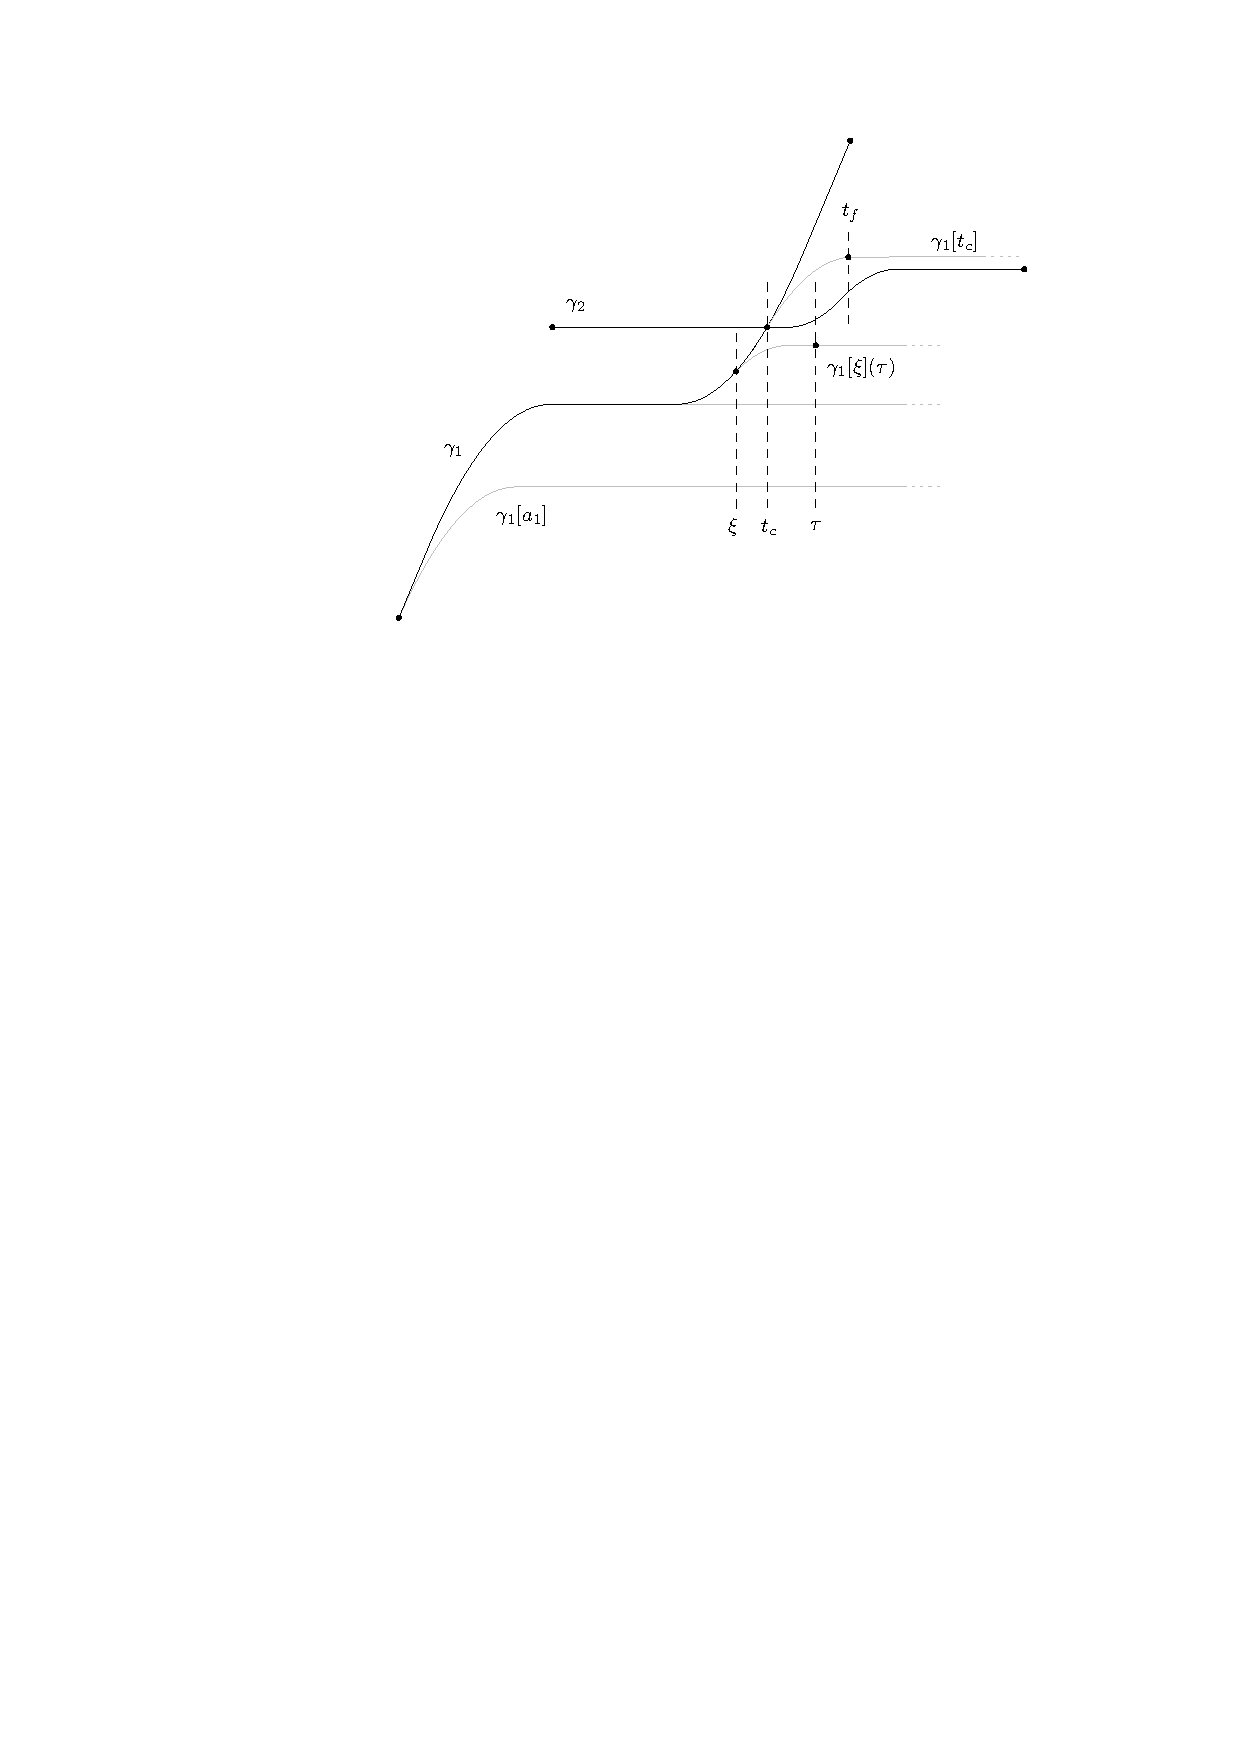
\includegraphics[scale=1.0]{figures/motion/rough/curvejoiningproof}
  \caption{Sketch of some quantities used in the proof of
    Lemma~\ref{lemma:curvejoining}, including some stopping trajectory
    candidates drawn in grey. The unique stopping trajectory satisfying the requirements of
    Lemma~\ref{lemma:curvejoining} is marked as $\varphi_{1}$.
    % The little open dot halfway on $\gamma_{2}$ is refered to in Remark~\ref{rem:conditions}.
  }%
  \label{fig:proof}
\end{figure}

\begin{proof}
  Define the set $U$ and the functions $X(t, x)$ and $\xi(t, x)$ as we did in \cref{eq:X,eq:xi,eq:U} for $\gamma$ above, but now for $\gamma_{1}$.
\begin{outline}

  % \1 Define $g$ such that $g(x, \tau) = \dot{\gamma}_{1}[\xi](\tau)$
  % for any $\xi$ such that $\gamma_{1}[\xi](\tau) = x$.

  % \2 Writing $h_{\tau}(\xi) := f_{x}(\xi, \tau)$, we define
  % $h_{\tau}^{-1}(x) := \{ \xi : f_{x}(\xi, \tau) = x \}$. Because this is the level set of a
  % continuous non-decreasing function, it must be a closed interval (Lemma~\ref{lemma:levelset}).
  % Hence, $g(x, \tau) := f_{v}(\max h_{\tau}^{-1}(x), \tau)$ is well-defined.

  \1 Identify for which parameters $\xi < t_{c} < \tau$ we have
  $\gamma_{1}[\xi](\tau) = \gamma_{2}(\tau)$ and $\dot{\gamma_{1}}[\xi](\tau) = \dot{\gamma}_{2}(\tau)$.

  \2 For each $\tau > t_{c}$, observe that $(\tau, \gamma_{2}(\tau)) \in U$. It follows
  from Property~\ref{prop:xi-unique} that
  $\varphi_{[\tau]} := \gamma_{1}[\xi(\tau, \gamma_{2}(\tau))]$ is the unique stopping trajectory such
  that $\varphi_{[\tau]}(\tau) = \gamma_{2}(\tau)$.
  %
  Next, we investigate when this unique trajectory touches $\gamma_{2}$
  tangentially. More precisely, consider the set of times
  \begin{align}
    T := \{ \tau > t_{c} : \dot{\varphi}_{[\tau]}(\tau) = \dot{\gamma}_{2}(\tau), \; \xi(\tau, \gamma_{2}(\tau)) < t_{c} \},
  \end{align}
  %
  which can also be written as
  \begin{align}
    T = \{ \tau > t_{c} : g(\tau, \gamma_{2}(\tau)) = \dot{\gamma}_{2}(\tau), \; \xi(\tau, \gamma_{2}(\tau)) < t_{c} \} ,
  \end{align}
  so continuity of $g$ shows that it is a closed set (Lemma~\ref{lemma:levelset}). It is not
  necessarily connected (see for example Figure~\ref{fig:proof}, in which $\varphi_{1}$ and
  $\varphi_{2}$ touch $\gamma_{2}$ tangentially on separated intervals). In
  general, $T$ is the union of a sequence of disjoint closed intervals
  $T_{1}, T_{2}, \dots, T_{n}$.

  \2 Define $\tau_{i} := \min \, T_{i}$ and let $\varphi_{i} := \varphi_{[\tau_{i}]}$
  denote the unique stopping trajectory through $(\tau_{i}, \gamma_{2}(\tau_{i}))$.
  %
  For $\tau \in T_{i}$, we have
  $\dot{\gamma}_{2}(\tau) = g(\tau, \gamma_{2}(\tau))$ by definition of $T_{i}$.
  %
  Moreover, we have
  \begin{align}\label{eq:phi-tangent}
    \dot{\varphi}_{i}(t) = g(t, \varphi_{i}(t)),
  \end{align}
  for every $t$ for which these quantities are defined, so in particular on $T_{i}$.
  %
  This shows that $\gamma_{2}$ and $\varphi_{i}$ are both solutions to the initial value problem
  \begin{align}
    \begin{cases}
      \,\dot{x}(t)\, = g(t, x(t)) \;  \text{ for } t \in T_{i} , \\
      x(\tau_{i}) = \gamma_{2}(\tau_{i}) .
    \end{cases}
  \end{align}
  %
  Since $g(t, x)$ is continuous in $t$ and Lipschitz continuous in $x$, it is a
  consequence of the (local) existence and uniqueness theorem
  (Lemma~\ref{lemma:picard}) that $\gamma_{2} = \varphi_{i}$ on $T_{i}$.
  %
  Hence, we have $\varphi_{i} = \varphi_{[\tau]}$ for any $\tau \in T_{i}$, so we regard
  $\varphi_{i}$ as being the canonical stopping trajectory for $T_{i}$.

  % Let $\tau'$ be the largest $\tau \in T_{i}$ such that
  % $\gamma_{2}(\tau) = \varphi_{i}(\tau)$. Suppose $\tau' < \hat{\tau}_{i}$, then by
  % the existence and uniqueness theorem (Picard-Lindel{\"o}f) there exists a
  % unique solution of the initial value problem
  % \begin{align*}
  %   \dot{\phi}(t) = g(t, \phi(t)), \quad \phi(\tau') = \gamma_{2}(\tau')
  % \end{align*}
  % on the interval $[\tau' - \delta, \tau' + \delta]$ for some $\delta > 0$.
  %
  % But $\varphi_{i}$ is a solution, so
  % $\varphi_{i}(\tau' + \delta) = \gamma_{2}(\tau' + \delta)$ for some sufficiently
  % small $\delta > 0$, but this contradicts the definition of $\tau'$. Therefore,
  % $\tau' = \hat{\tau}_{i}$.

  % \1 Next, we show that $\tau_{1}$ and thus $\varphi_{1}$ exists.
  % % and $t_{f} := t_{c} + \dot{\gamma}_{1}(t_{c}) / \omega$.
  % This part relies on conditions (C1) and (C2).
  % %
  % Note that $s(\tau) := g(\tau, \gamma_{2}(\tau))$ is a continuous function.
  % %
  % We have $\gamma_{1}[a_{1}](t) \leq \gamma_{2}(t) \leq \gamma_{1}[t_{c}](t)$ for
  % $t \in \{ t_{c}, b_{2} \}$, so the intermediate value theorem guarantees that
  % $s(t)$ actually exists in both cases, because there is some
  % $a_{1} \leq \xi < t_{c}$ such that $\gamma_{2}(t) = \gamma_{1}[\xi](t)$ and thus
  % $s(t) = g(t, \gamma_{2}(t)) = \dot{\gamma}_{1}[\xi](t)$ exists.
  % %
  % We have $\dot{\gamma}_{2}(t_{c}) < \dot{\gamma}_{1}(t_{c}) = s(t_{c})$ and
  % $\dot{\gamma}_{2}(b_{2}) = 1 \geq s(b_{2})$, so there must be some smallest
  % $\tau_{1} \in \openhalf{t_{c}}{b_{2}}$ such that
  % $\dot{\gamma}_{1}(\tau_{1}) = s(\tau_{1})$, as a consequence of the
  % intermediate value theorem.

  % \2 Suppose $\gamma_{2}(t_{f}) \leq \gamma_{1}[t_{c}](t_{f})$, then it follows from the fact
  % that $g$ is non-decreasing in $x$ that
  % $g(t_{f}, \gamma_{2}(t_{f})) \leq g(t_{f}, \gamma_{1}[t_{c}](t_{f})) = \dot{\gamma}_{1}(t_{c}) - \omega(t_{f} - t_{c}) = 0$,
  % so $s(t_{f}) = 0$.

  % \2 Otherwise $\gamma_{2}(t_{f}) > \gamma_{1}[t_{c}](t_{f})$, then it follows
  % (from Lemma \dots) that $\gamma_{2}$ crosses $\gamma_{1}[t_{c}]$ at some time
  % $t_{d} \in (t_{c}, t_{f})$ with
  % $\dot{\gamma}_{2}(t_{d}) > \gamma_{1}[t_{c}](t_{d}) = s(t_{d})$.

  % \2 We have $\gamma_{1}[a_{1}](t) \leq \gamma_{2}(t) \leq \gamma_{1}[t_{c}](t)$ for
  % $t \in \{ t_{f}, t_{d} \}$, so the intermediate value theorem guarantees that
  % $s(t)$ actually exists in both cases, because there is some
  % $a_{1} \leq \xi < t_{c}$ such that $\gamma_{2}(t) = \gamma_{1}[\xi](t)$ and thus
  % $s(t) = g(t, \gamma_{2}(t)) = \dot{\gamma}_{1}[\xi](t)$ exists.

  % \2 In both cases above, we have
  % $\dot{\gamma}_{2}(t_{c}) < \dot{\gamma}_{1}(t_{c}) = s(t_{c})$ and
  % $\dot{\gamma}_{2}(t_{d}) \geq s(t_{d})$ for some $t_{d} \in \openhalf{t_{c}}{t_{f}}$.
  % Hence, there must be some smallest $\tau_{1} \in \openhalf{t_{c}}{t_{d}}$ such that
  % $\dot{\gamma_{2}}(\tau_{1}) = s(\tau_{1})$, which is a consequence of the intermediate
  % value theorem.

  \1 If $i \geq 2$, then $\varphi_{i} > \gamma_{2}$ somewhere.

  \2 Let $i \geq 1$, we show that $\varphi_{i+1}(t) > \gamma_{2}(t)$ for some $t$.
  %
  Recall the lower bound property, so $\gamma_{2}(t) \geq \varphi_{i}(t)$ and
  $\dot{\gamma}_{2}(t) \geq \dot{\varphi}_{i}(t)$ for $t \geq \tau_{i}$.
  %
  Define $\hat{\tau}_{i} := \max \, T_{i}$, such that
  $T_{i} = [\tau_{i}, \hat{\tau}_{i}]$, then by definition of $T_{i}$, there
  must be some $\delta > 0$ such that
  \begin{align}
    \gamma_{2}(\hat{\tau}_{i} + \delta) > \varphi_{i}(\hat{\tau}_{i} + \delta) ,
  \end{align}
  since otherwise $\gamma_{2} = \varphi_{i}$ on some open neighborhood of
  $\hat{\tau}_{i}$ and then also
  \begin{align}
    \dot{\gamma}_{2}(t) = \dot{\varphi}_{i}(t) \overset{\text{\eqref{eq:phi-tangent}}}{=} g(t, \varphi_{i}(t)) = g(t, \gamma_{2}(t)),
  \end{align}
  which contradicts the definition of $\hat{\tau}_{i}$.
  %
  Therefore, we have $\gamma_{2}(t) > \varphi_{i}(t)$ for all $t \geq \hat{\tau}_{i} + \delta$. For
  $t = \tau_{i+1}$, in particular, it follows that
  $\varphi_{i+1}(\tau_{i+1}) = \gamma_{2}(\tau_{i+1}) > \varphi_{i}(\tau_{i+1})$, which shows that
  $\varphi_{i+1} > \varphi_{i}$ on $(\xi_{i}, \infty)$, due to Property~\ref{prop:xi-unique}, but this means that
  $\varphi_{i+1}(\tau_{i}) > \varphi_{i}(\tau_{i}) = \gamma_{2}(\tau_{i})$.

  \1 If $\varphi_{i} > \gamma_{2}$ somewhere, then $i \geq 2$.

  \2 Suppose $\varphi_{i}(t_{x}) > \gamma_{2}(t_{x})$ for some
  $t_{x} \in (t_{c}, \tau_{i})$, then there must be some
  $\tau_{0} \in (t_{c}, t_{x})$ such that
  $\gamma_{2}(\tau_{0}) = \varphi_{i}(\tau_{0})$ and
  $\dot{\gamma}_{2}(\tau_{0}) < \dot{\varphi}(\tau_{0})$. Note that this
  crossing must happen because we require $\xi_{i} < t_{c}$.

  \2 Since $g(t, x)$ is non-decreasing in $x$, we have
  \begin{align}
    s(t) = g(t, \gamma_{2}(t)) \leq g(t, \varphi_{i}(t)) = \dot{\varphi}_{i}(t) ,
  \end{align}
  for every $t \in [\tau_{0}, \tau_{i}]$ and at the endpoints, we have
  \begin{align}
    s(\tau_{0}) = \varphi_{i}(\tau_{0}), \quad s(\tau_{i}) = \varphi_{i}(\tau_{i}) .
  \end{align}
  %
  Furthermore, observe that $\gamma_{2}(\tau_{0}) = \varphi_{i}(\tau_{0})$ and
  $\gamma_{2}(\tau_{i}) = \varphi_{i}(\tau_{i})$ require that
  \begin{align}\label{eq:distance-traveled}
    \int_{\tau_{0}}^{\tau_{i}} \dot{\gamma}_{2}(t) \diff t  = \int_{\tau_{0}}^{\tau_{i}} \dot{\varphi}_{i}(t) \diff t .
  \end{align}

  \2 Since $\dot{\gamma}_{2}(\tau_{0}) < \dot{\varphi}_{i}(\tau_{0})$, it follows
  from~\eqref{eq:distance-traveled} that there must be some $t \in (\tau_{0}, \tau_{i})$
  such that $\dot{\gamma}_{2}(t) > \dot{\varphi}_{i}(t)$.
  %
  Together with $s(\tau_{0}) = \dot{\varphi}_{i}(\tau_{0}) > \dot{\gamma}_{2}(\tau_{0})$
  and $s(t) \leq \dot{\varphi}_{i}(t)$ for $t \in [\tau_{0}, \tau_{i}]$, this means there is some $\tau^{*}$ such
  that $\dot{\gamma}_{2}(\tau^{*}) = s(\tau^{*})$, again as a consequence of the
  intermediate value theorem. Therefore, $\tau^{*} \in T_{j}$ for some $j < i$, which
  shows that $i \geq 2$.


  \1 The above two points establish that $\varphi_{i} \leq \gamma_{2}$ if and only if $i=1$.
  To conclude, we have shown that if $\varphi := \varphi_{1}$ exists, it is the unique
  trajectory satisfying the stated requirements with $\tau = \tau_{i}$ and
  $\xi = \xi(\tau_{i}, \gamma_{2}(\tau_{i}))$. \qedhere
\end{outline}
\end{proof}


% \begin{remark}\label{rem:conditions}
%   It is easy to see that condition (C1) in Lemma~\ref{lemma:curvejoining} is necessary. Suppose there
%   is some $t_{x} \in (t_{c}, \infty)$ such that
%   $\gamma_{1}[a_{1}](t_{x}) > \gamma_{2}(t_{x})$, then for any other
%   $\xi \in (a_{1}, t_{c})$, we have $\gamma_{1}[\xi](t_{x}) > \gamma_{2}(t_{x})$
%   as well, due to the lower bound property of stopping trajectories, so
%   requirement \textit{(iii)} is violated.
%   %
%   Condition (C2) is not necessary, which can be seen from stopping trajectory
%   $\varphi_{1}$ in Figure~\ref{fig:proof}, which satisfies the conditions, but
%   would also have been valid if $\gamma_{2}$ ended somewhat earlier than
%   $t_{f}$, for example until the open dot.
% \end{remark}

The uniqueness result justifies the following definition of joined trajectories.

\begin{define}
  Let $\gamma_{1} \in \mathcal{D}[a_{1}, b_{1}]$ and
  $\gamma_{2} \in \mathcal{D}[a_{2}, b_{2}]$ and suppose they intersect at
  exactly a single time $t_{c}$. We write $\gamma_{1} * \gamma_{2}$ to denote
  the unique \emph{joined trajectory}
  \begin{align}
    (\gamma_{1} * \gamma_{2})(t) =
    \begin{cases}
      \gamma_{1}(t) & \text{ for } t < \xi , \\
      \gamma_{1}[\xi](t) & \text{ for } t \in [\xi, \tau] , \\
      \gamma_{2}(t) & \text{ for } t > \tau ,
    \end{cases}
  \end{align}
  satisfying $\gamma_{1} * \gamma_{2} \in \mathcal{D}[a_{1}, b_{2}]$, when it exists.
  %
  If $\dot{\gamma}_{1}(t_{c}) = \dot{\gamma}_{2}(t_{c})$, then we define $\tau=\xi=t_{c}$.
\end{define}

Next, we discuss existence of joined trajectories.

\begin{lemma}
  Let $\gamma_{1} \in \mathcal{D}[a_{1}, b_{1}]$ and
  $\gamma_{2} \in \mathcal{D}[a_{2},b_{2}]$. If there is some trajectory
  $\mu \in \mathcal{D}[a_{1}, b_{2}]$ such that
  $\mu \leq \min\{\gamma_{1}, \gamma_{2}\}$ and
  \begin{align*}
    \mu(a_{1}) = \gamma_{1}(a_{1}), \quad \mu(b_{2}) = \gamma_{2}(b_{2}), \\
    \dot{\mu}(a_{1}) = \dot{\gamma}_{1}(a_{1}), \quad \dot{\mu}(b_{2}) = \dot{\gamma_{2}}(b_{2}).
  \end{align*}
  then $\gamma_{1} * \gamma_{2}$ exists.
\end{lemma}
\begin{proof} {\color{Navy} Still todo, but I can adapt an earlier version of
    this argument, which was previously part of Lemma 1.}
\end{proof}


Our main interest in $\gamma_{1} * \gamma_{2}$ is due to the following upper bounding
property.

\begin{lemma}\label{lemma:upperbound}
  Let $\gamma_{1} \in \mathcal{D}[a_{1}, b_{2}]$ and
  $\gamma_{2} \in \mathcal{D}[a_{2}, b_{2}]$ be such that $\gamma_{1} * \gamma_{2}$ exists. All
  trajectories $\mu \in \mathcal{D}[a, b]$ that are such that
  $\mu \leq \min\{\gamma_{1}, \gamma_{2}\}$, must satisfy $\mu \leq \gamma_{1} * \gamma_{2}$.
\end{lemma}
\begin{proof}
  Write $\gamma := \gamma_{1} * \gamma_{2}$ as a shorthand. We obviously have
  $\mu \leq \gamma$ on $[a_{1}, \xi] \cup [\tau, b_{2}]$, so consider the interval $(\xi, \tau)$ of the joining
  deceleration part. Suppose there exists some $t_{d} \in (\xi, \tau)$ such that
  $\mu(t_{d}) > \gamma(t_{d})$. Because $\mu(\xi) \leq \gamma(\xi)$, this means that $\mu$ must
  intersect $\gamma$ at least once in $\halfopen{\xi}{t_{d}}$, so let
  $t_{c} := \sup \, \{ t \in \halfopen{\xi}{t_{d}} : \mu(t) = \gamma(t) \}$ be the latest
  time of intersection such that $\mu \geq \gamma$ on $[t_{c}, t_{d}]$. There must be
  some $t_{c} \in [t_{c}, t_{d}]$ such that $\dot{\mu}(t_{v}) > \dot{\gamma}(t_{v})$, otherwise
  \begin{align*}
    \mu(t_{d}) = \mu(t_{c}) + \int_{t_{c}}^{t_{d}} \dot{\mu}(t) \diff t \leq \gamma(t_{c}) + \int_{t_{c}}^{t_{d}} \dot{\gamma}(t) \diff t = \gamma(d_{t}) ,
  \end{align*}
  which contradicts our choice of $t_{d}$. Hence, for every
  $t \in [t_{v}, \tau]$, we have
  \begin{align*}
    \dot{\mu}(t) \geq \dot{\mu}(t_{v}) - \omega (t - t_{v}) > \dot{\gamma}(t_{v}) - \omega(t - t_{v}) = \dot{\gamma}(t) .
  \end{align*}
  It follows that $\mu(\tau) > \gamma(\tau)$, which contradicts
  $\mu \leq \gamma_{2}$.
\end{proof}



\newpage
\appendix
\section{Miscellaneous}

\begin{lemma}\label{lemma:levelset}
  Let $f :\mathbb{R}^{n} \rightarrow \mathbb{R}^{m}$ be continuous and
  $y \in \mathbb{R}^{m}$, then the level set $N := f^{-1}(\{ y \})$ is a closed
  subset of $\mathbb{R}^{n}$.
\end{lemma}
\begin{proof}
  For any $y' \neq y$, there exists an open neighborhood $M(y')$ such that
  $y \notin M(y')$. The preimage $f^{-1}(M(y'))$ is open by continuity.
  Therefore, the complement
  $N^{c} = \{ x : f(x) \neq y \} = \cup_{y' \neq y} f^{-1}(\{y'\}) = \cup_{y' \neq y} f^{-1}(M(y'))$
  is open.
\end{proof}

\begin{lemma}\label{lemma:picard}
  Let $D \subseteq \mathbb{R} \times \mathbb{R}^{n}$ be some closed rectangle such that
  $(t_{0}, x_{0}) \in \interior D$.
  Let $f : D \rightarrow \mathbb{R}^{n}$ be a function that is continuous in $t$
  and globally Lipschitz continuous in $x$, then there exists some $\varepsilon > 0$
  such that the initial value problem
  \begin{align}
    \label{eq:1}
    \dot{x}(t) = f(t, x(t)), \quad x(t_{0}) = x_{0}
  \end{align}
  has a unique solution $x(t)$ on the interval
  $[t_{0} - \varepsilon, t_{0} + \varepsilon]$.
\end{lemma}

{\color{Navy} The above existence and uniqueness theorem is also known as the
  Picard-Lindel{\"o}f or Cauchy-Lipschitz theorem. The above statement is based
  on the Wikipedia page on this theorem, so we still need a slightly better
  reference.}

\begin{lemma}\label{lemma:inf-continuous}
  Let $f : X \times Y \rightarrow \mathbb{R}$ be some continuous function. If
  $Y$ is compact, then the function $g : X \rightarrow \mathbb{R}$, defined as
  $g(x) = \inf \{ f(x,y) : y\in Y\}$, is also continuous.
\end{lemma}

\end{document}

% to enable the minted package
% Local Variables:
% TeX-command-extra-options: "-shell-escape"
% End:
